\documentclass[a4paper]{article}

% Basic packages
\usepackage{fontspec}
\XeTeXlinebreaklocale "zh"    % 启用中文断行（XeTeX 内建，无需 xeCJK）
\XeTeXlinebreakskip = 0pt plus 1pt
\setmainfont{Songti SC}
\setsansfont{Heiti SC}
\setmonofont{Menlo}
\usepackage{amsmath, amssymb}
\usepackage{graphicx}
\usepackage[margin=2.5cm]{geometry}
\usepackage[most]{tcolorbox}
\usepackage{etoolbox}
\usepackage{listings}
\usepackage{hyperref}
\usepackage{booktabs}
\usepackage{subcaption}
\usepackage{float}

% Chinese font setup (macOS system fonts, no ctex needed)
\setmainfont{Songti SC}
\setsansfont{Heiti SC}
\setmonofont{Menlo}
\newcommand{\song}{\fontspec{Songti SC}}
\newcommand{\hei}{\fontspec{Heiti SC}}
\newcommand{\kai}{\fontspec{KaiTi}}
\newcommand{\fangsong}{\fontspec{FangSong}}

% ===== Highlight boxes =====
\newtcolorbox{knowledgebox}[1]{
    enhanced, colback=blue!5!white, colframe=blue!75!black, colbacktitle=blue!75!black,
    coltitle=white, fonttitle=\bfseries, title=#1, attach boxed title to top left={yshift=-2mm, xshift=2mm},
    boxrule=1pt, sharp corners
}

\newtcolorbox{importantbox}[1]{
    enhanced, colback=yellow!10!white, colframe=yellow!80!black, colbacktitle=yellow!80!black,
    coltitle=black, fonttitle=\bfseries, title=#1, sharp corners
}

\newtcolorbox{warningbox}[1]{
    enhanced, colback=red!5!white, colframe=red!75!black, colbacktitle=red!75!black,
    coltitle=white, fonttitle=\bfseries, title=#1, sharp corners
}

\newtcolorbox{practicebox}[1]{
    enhanced, colback=green!5!white, colframe=green!60!black, colbacktitle=green!60!black,
    coltitle=white, fonttitle=\bfseries, title=#1, sharp corners
}

% ===== Code listings =====
\lstset{
    basicstyle=\ttfamily\small,
    keywordstyle=\color{blue},
    stringstyle=\color{red!60!black},
    commentstyle=\color{green!60!black},
    breaklines=true,
    frame=single,
    numbers=left,
    numberstyle=\tiny\color{gray},
    captionpos=b,
    extendedchars=false
}

% ===== Front-page metadata =====
\newcommand{\notetitle}{CS336 Lecture 13：语言建模的数据（Data 1）}
\newcommand{\notesubtitle}{Stanford CS336: Language Modeling from Scratch (Spring 2025)}
\newcommand{\noteauthors}{讲师：Percy Liang, Tatsu Hashimoto \quad 笔记：ZCode}
\newcommand{\notedate}{2026-07-14}
\newcommand{\videochannel}{Stanford CS336}
\newcommand{\videopublishdate}{2025 Spring}
\newcommand{\videoduration}{79 分钟}
\newcommand{\videourl}{https://www.youtube.com/watch?v=SQ3fZ1sAqXI}
\newcommand{\videocoverpath}{cover.jpg}

\begin{document}

% ===== Title page =====
\begin{titlepage}
\centering
{\Large 课程笔记\par}
\vspace{1.2cm}
{\huge\bfseries \notetitle\par}
\vspace{0.3cm}
{\large \notesubtitle\par}
\vspace{0.5cm}
{\large \noteauthors\par}
\vspace{0.3cm}
{\large \notedate\par}
\vspace{1.0cm}

\includegraphics[width=0.82\textwidth,height=0.40\textheight,keepaspectratio]{\videocoverpath}\par

\vfill
\begin{tcolorbox}[width=0.9\textwidth, colback=black!2!white, colframe=black!60, sharp corners]
\textbf{视频作者/频道}：\videochannel\par
\textbf{发布日期}：\videopublishdate\par
\textbf{视频时长}：\videoduration\par
\textbf{视频链接}：\href{\videourl}{\nolinkurl{\videourl}}
\end{tcolorbox}
\end{titlepage}

\tableofcontents
\newpage

%% --- 正文内容开始 ---

\section{数据为什么是语言模型的核心}

\subsection{一个挑衅性的论断：数据最重要}

在前面的课程里，我们一直在讨论\emph{给定固定数据集}如何训练模型——架构、优化器、分词、scaling laws、并行化。本讲起，我们终于要回答一个更根本的问题：\textbf{到底该用什么数据来训练？}

Percy Liang 开篇就抛出一个"hot take"：

\begin{importantbox}{核心论断}
数据（data）是把语言模型做对的最重要因素。Tatsu 可能不同意——他认为 scaling laws 才是最重要的。但 Percy 给出的论证来自工业界的真实披露行为。
\end{importantbox}

\begin{figure}[H]
\centering
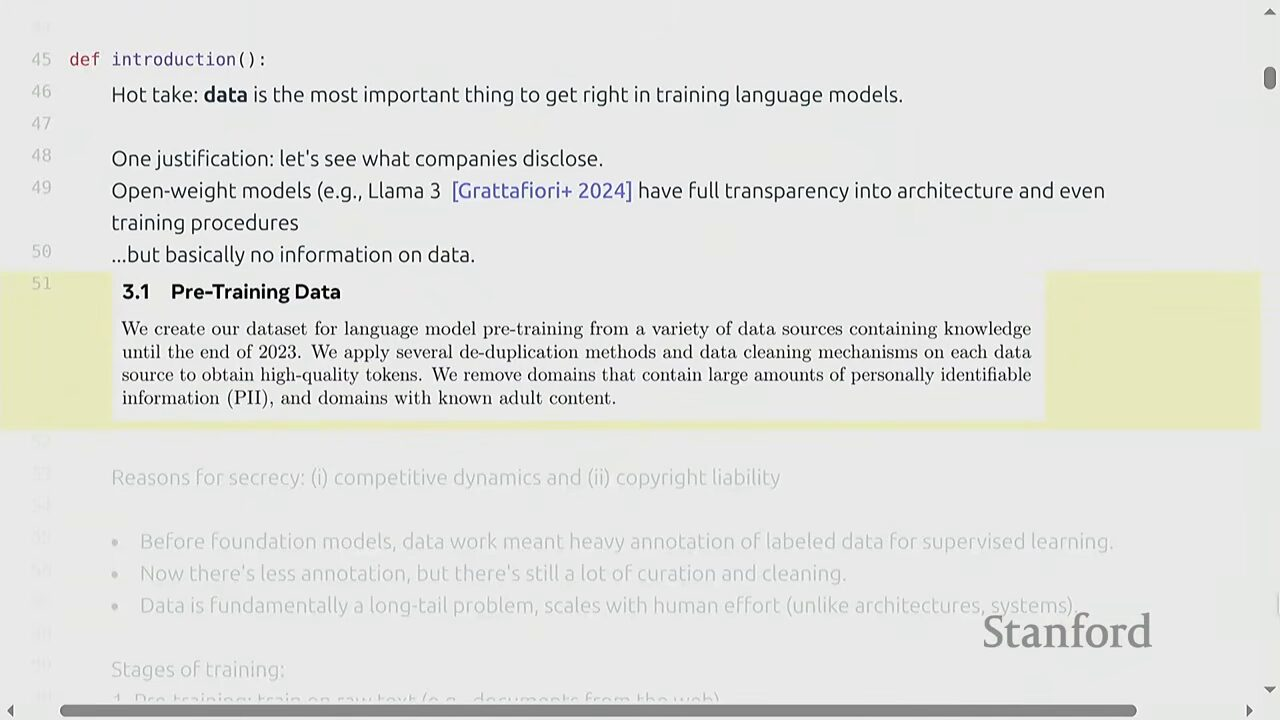
\includegraphics[width=0.92\textwidth]{figures/fig_01_intro.jpg}
\caption{本讲的中心命题：数据是语言模型质量的决定性因素\protect\footnotemark}
\end{figure}
\footnotetext{视频画面时间区间：00:00:40--00:01:20。}

\subsection{来自工业界的间接证据：保密的就是数据}

如果你去读 Llama 3、DeepSeek 这些 open-weight 模型的论文，会发现一个有趣的不对称：

\begin{itemize}
\item \textbf{架构}：完全公开，细节详尽（层数、注意力头、激活函数、归一化方式……）。
\item \textbf{训练流程}：也讲得相当多（优化器配置、学习率调度、batch size 增长策略……）。
\item \textbf{数据}：几乎只字不提。Llama 3 论文里关于数据，全部内容大致就是一句"We create our data set from a variety of data sources containing knowledge until the end of 2023"。
\end{itemize}

\begin{knowledgebox}{为什么数据被保密？}
两个原因：\textbf{(1) 竞争动态}——数据配方是真正的护城河；\textbf{(2) 法律风险}——不想在已有的版权诉讼火上再浇油。在 foundation model 时代之前，数据的重要性是显而易见的（监督学习需要标注）；如今虽然标注少了，但\emph{数据的策展与清洗}（curation and cleaning）依然是海量工作。数据是一条"长尾"问题，而且\textbf{可并行性极强}：你可以轻松雇几百人分别处理多语言、代码、图像等不同方面，而架构只需要一个小团队定一次。
\end{knowledgebox}

\subsection{训练的三个阶段}

语言模型的训练通常分为三个阶段，质量从低到高、数量从大到小：

\begin{tcolorbox}[enhanced, colback=black!2!white, colframe=black!60, sharp corners, title=\textbf{训练阶段与数据特征}]
\begin{description}
\item[Pre-training（预训练）] 在海量原始网页数据上训练，本课的主要焦点。数据量级在万亿 tokens。
\item[Mid-training（中期训练）] 在精选的高质量子集上继续训练，针对特定能力（数学、代码、长上下文）。量级约百亿到千亿 tokens。
\item[Post-training（后训练）] 在指令跟随 / 对话数据上微调，或用 RLHF。安全对齐通常也在这里。
\end{description}
\end{tcolorbox}

\textbf{基本直觉}：从大量低质量数据开始，逐步过渡到少量高质量数据。实践中三者界限模糊，最近的模型阶段越来越多。\textbf{Base model} 通常指 pre-training + mid-training 后的检查点；\textbf{chat / instruct model} 指再经过 post-training 的版本。

\subsection{一个具体例子：AI2 OLMo 的数据混合}

为了把这些抽象阶段落到实处，Percy 展示了 AI2（Allen Institute for AI）OLMo 系列模型的真实数据配比——因为 AI2 完全开源，我们能确切知道数据里有什么。

\begin{figure}[H]
\centering
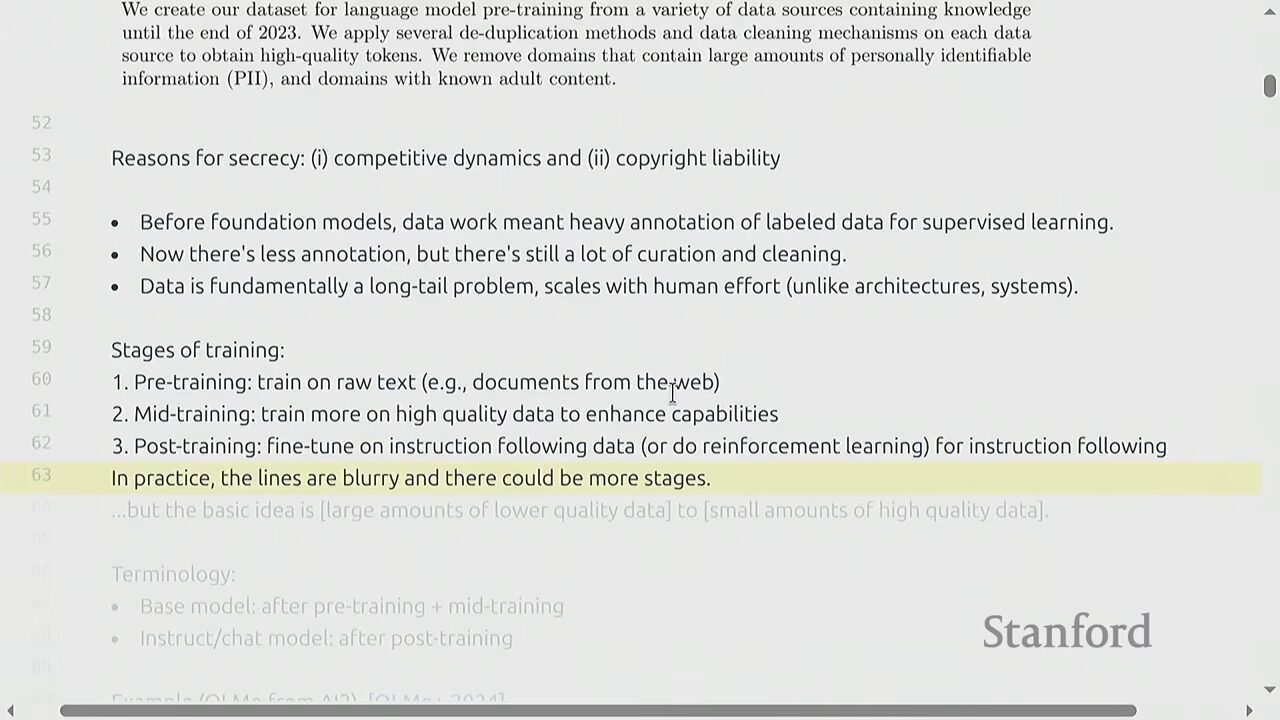
\includegraphics[width=0.95\textwidth]{figures/fig_02_ai2_mix.jpg}
\caption{OLMo 的典型预训练数据混合：DCLM baseline、代码、论文、数学、Wikipedia，合计约 3.9T tokens\protect\footnotemark}
\end{figure}
\footnotetext{视频画面时间区间：00:03:30--00:04:30。}

预训练阶段约 \textbf{3.9T tokens}，主要来源是 DCLM baseline（一种过滤后的 Common Crawl）、代码、学术论文、数学语料和 Wikipedia。到了 mid-training，同样是这些来源但被\emph{大幅过滤}——DCLM 从 3.7T 砍到 700B，再叠加 FLAN、Wikipedia、合成数据、GSM8K，总计约 10B tokens。Post-training 则是另一套（Tulu）配方，主要是各种聊天数据和合成数据。

\begin{warningbox}{本讲的诚实声明}
关于"这些数据集是怎么选的、怎么处理的"，\textbf{并没有一套正式的原则或理论}。Percy 坦言：数据是最难教的部分，因为"教数据"到底意味着什么都不清楚。所以本讲的策略是：带你纵览历年来人们用过的数据集，讲清它们的来源和性质，让你自己用归纳能力建立"什么才是好数据"的直觉。
\end{warningbox}

\section{早期数据集：从 BERT 到 GPT-2}

我们把时间拨回 2018 年，沿着数据集的演化脉络一路走到今天。这条时间线揭示了数据工程是如何从"随便抓点文本"演变成一门精密工艺的。

\subsection{BERT（2018）：Books Corpus + Wikipedia}

\begin{figure}[H]
\centering
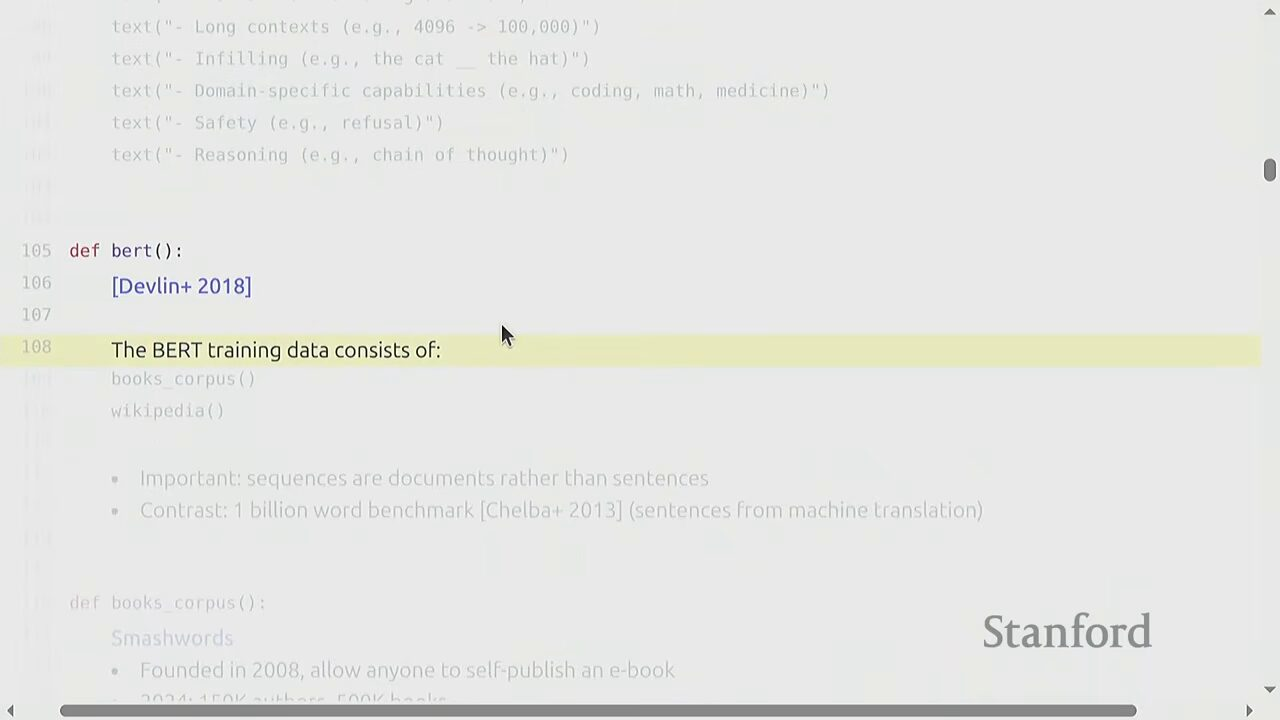
\includegraphics[width=0.92\textwidth]{figures/fig_03_bert.jpg}
\caption{BERT 的训练数据：Books Corpus 与 Wikipedia\protect\footnotemark}
\end{figure}
\footnotetext{视频画面时间区间：00:06:45--00:07:30。}

BERT 在今天看来很老，但它标志着一个重要转变：\textbf{从在句子上训练转向在完整文档上训练}（对比上周讲的 Billion Word Benchmark，那个时代是按句子切的）。它的两个数据源是：

\begin{itemize}
\item \textbf{Books Corpus}：来自 \texttt{Smashwords} 这个 2008 年上线的自助电子书出版平台。2015 年有一篇视觉-语言论文爬取了 Smashwords 上定价为零的自出版书籍，得到约 7,000 本。这个数据集后来因违反服务条款被下线——2015 年那会儿还是"狂野西部"，AI 版权远不是现在这个敏感话题。
\item \textbf{Wikipedia}：详见下一小节。
\end{itemize}

\subsection{Wikipedia：被神化的高质量来源}

\begin{figure}[H]
\centering
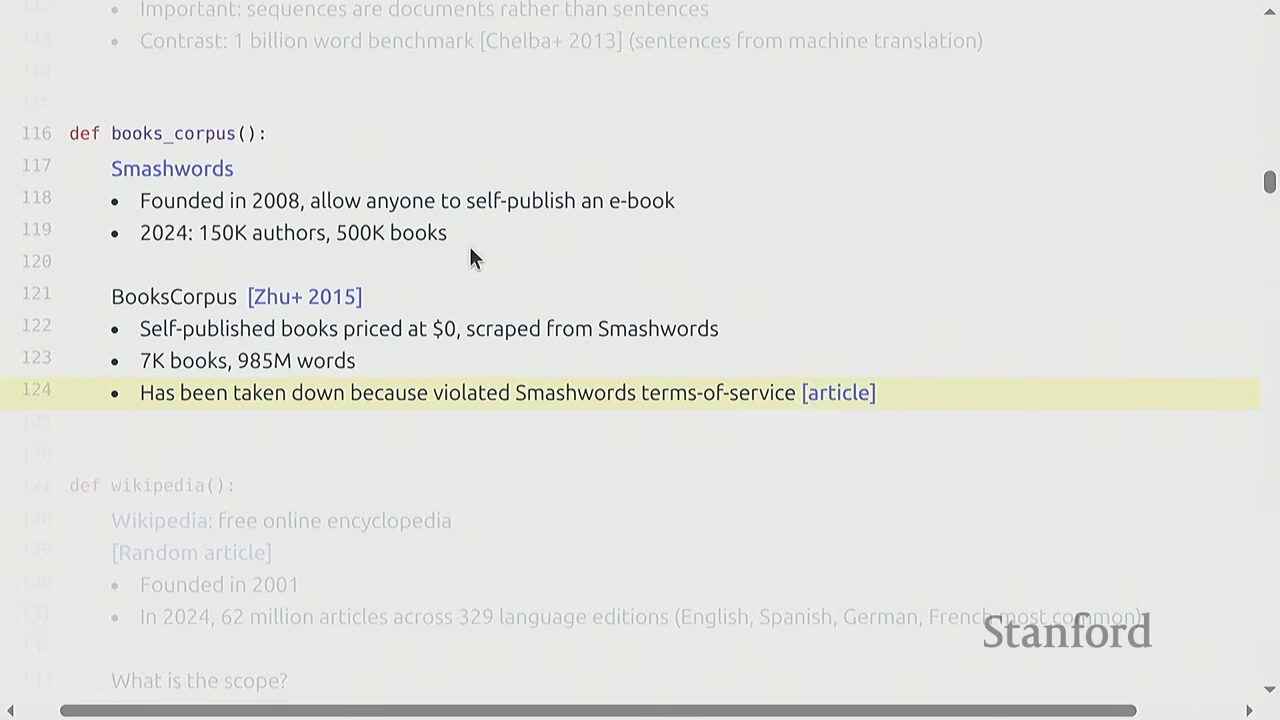
\includegraphics[width=0.92\textwidth]{figures/fig_04_wikipedia.jpg}
\caption{Wikipedia 的核心性质：可引用、基于 notability、任何人可编辑\protect\footnotemark}
\end{figure}
\footnotetext{视频画面时间区间：00:08:00--00:08:45。}

Wikipedia 存在了 20 多年，几乎每种语言都有大量条目。但要在数据语境下理解它，必须明确它的几条性质：

\begin{enumerate}
\item \textbf{不含原创思想}：所有内容必须来自可引用的一手/二手来源（所以条目里满是引用标记）。
\item \textbf{基于 notability}：一个主题必须有多个独立来源报道过，才会被收录。
\item \textbf{任何人可编辑}：但实践中是少数人贡献了绝大多数编辑（有人累计编辑达 500 万次，估计用了自动化工具）。
\item \textbf{定期 dump}：每隔一段时间发布一个打包好的压缩文件，可以整体下载。
\end{enumerate}

\begin{importantbox}{Wikipedia 的盲区}
正因为 notability 和"无原创"这两条，Wikipedia \textbf{系统性缺失}两类内容：长尾的、未被多家媒体覆盖的主题（也许很有价值）；以及观点性、操作性内容（比如菜谱就不在 Wikipedia 里）。这解释了为什么仅靠 Wikipedia 训不出好模型——它只是"高质量"的一个\emph{代理}（surrogate），而非全集。
\end{importantbox}

\subsection{数据投毒：Wikipedia 的安全漏洞}

\begin{figure}[H]
\centering
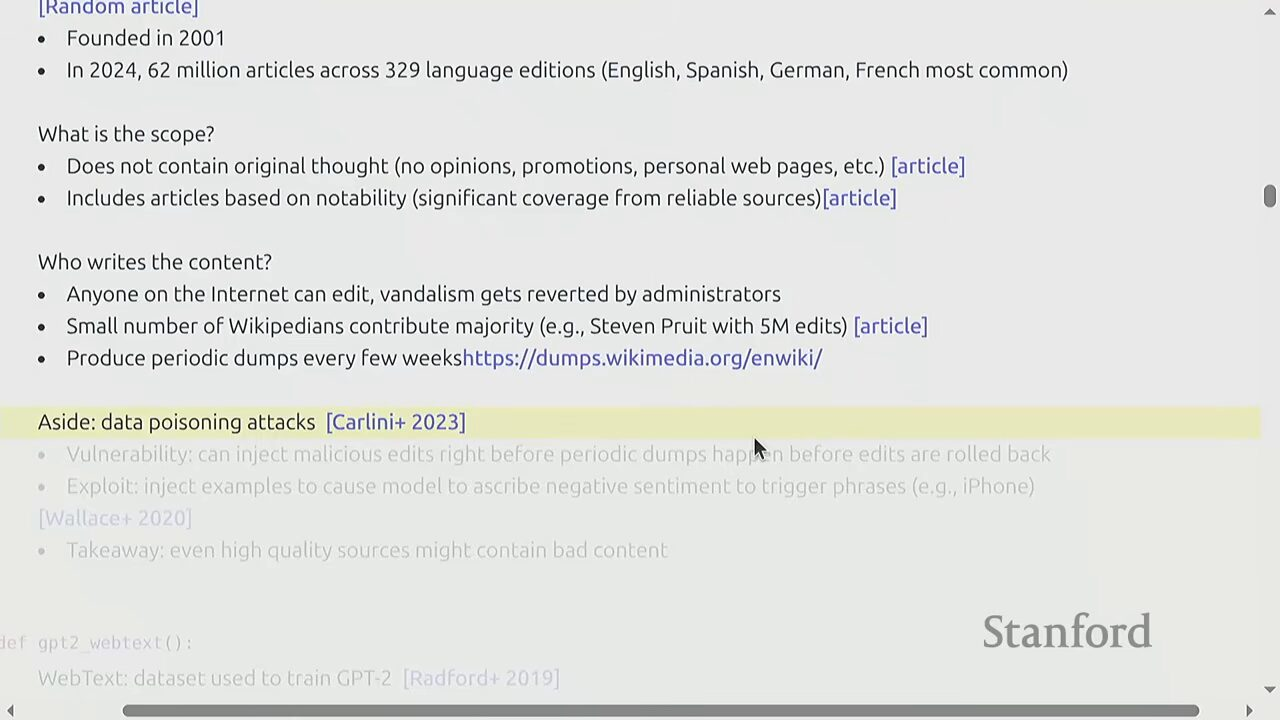
\includegraphics[width=0.92\textwidth]{figures/fig_05_poisoning.jpg}
\caption{Carlini 等人展示的数据投毒攻击：在 dump 发布前注入恶意编辑\protect\footnotemark}
\end{figure}
\footnotetext{视频画面时间区间：00:10:15--00:11:00。}

Nicholas Carlini 有一系列"一切都很脆弱"的研究，其中展示了针对 Wikipedia dump 的攻击：

\begin{tcolorbox}[enhanced, colback=red!5!white, colframe=red!75!black, sharp corners, title=\textbf{投毒攻击的时序}]
攻击者监视 dump 发布时间表，在 dump 即将生成前提交一条恶意编辑。由于社区审核需要时间，这条编辑会\emph{先进入 dump}，然后才被回滚。结果：dump 里留下了投毒内容。已知若能控制训练数据，就能让模型学到指定行为——比如对某个触发词（如"iPhone"）赋予负面情感。
\end{tcolorbox}

虽然 Wikipedia 后来打了补丁、这种具体利用已不奏效，但教训是深刻的：

\begin{warningbox}{更广泛的威胁模型}
模型训练数据来自开放的互联网，而攻击者与各种利益相关方对这些数据有\textbf{相当大的控制权}。对这一过程的监督极其困难。任何声称"我们的模型在互联网上训练"的声明，都隐含了一长串无法审计的中间环节。
\end{warningbox}

\subsection{GPT-2（2019）：WebText 与 Reddit karma 过滤}

GPT-2 的数据集叫 \textbf{WebText}，核心洞察是：互联网又大又乱，怎么快速拿到一个多样且高质量的子集？

答案是 \textbf{Reddit}。Reddit 上有大量外链，帖子可以获得 karma 点数。WebText 的做法是：只保留那些来自 karma $\geq 3$ 的帖子的外链指向的页面。结果是 800 万页面、约 \textbf{40 GB 文本}。

OpenAI 除了论文外\textbf{没有发布}这个数据集。后来社区有了开源复刻版 \textbf{OpenWebText}，在语言模型研究中被广泛使用。

\begin{knowledgebox}{一个反复出现的模式：用链接结构定位高质量内容}
WebText 的"karma $\geq 3$"和后面会讲的 LLaMA"被 Wikipedia 引用的页面"，本质上是同一种思想：\textbf{不直接判断页面质量，而是借助某种外部的质量信号（社交投票、权威来源的引用）来间接筛选}。这种"借力"策略在数据工程里反复出现。
\end{knowledgebox}

\section{Common Crawl：互联网的学术近似}

\subsection{Common Crawl 是什么}

\begin{figure}[H]
\centering
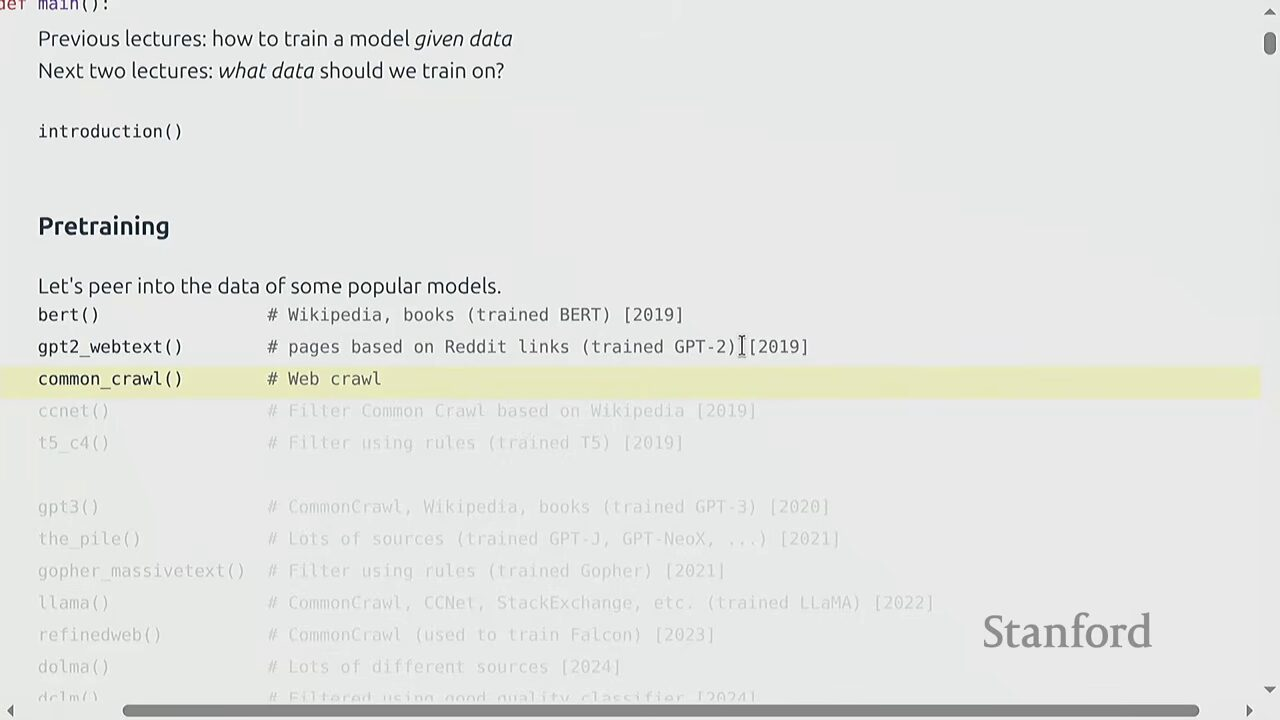
\includegraphics[width=0.95\textwidth]{figures/fig_06_commoncrawl.jpg}
\caption{Common Crawl：自 2007 年起每月一次的开放网页爬取\protect\footnotemark}
\end{figure}
\footnotetext{视频画面时间区间：00:13:30--00:14:15。}

\begin{figure}[H]
\centering
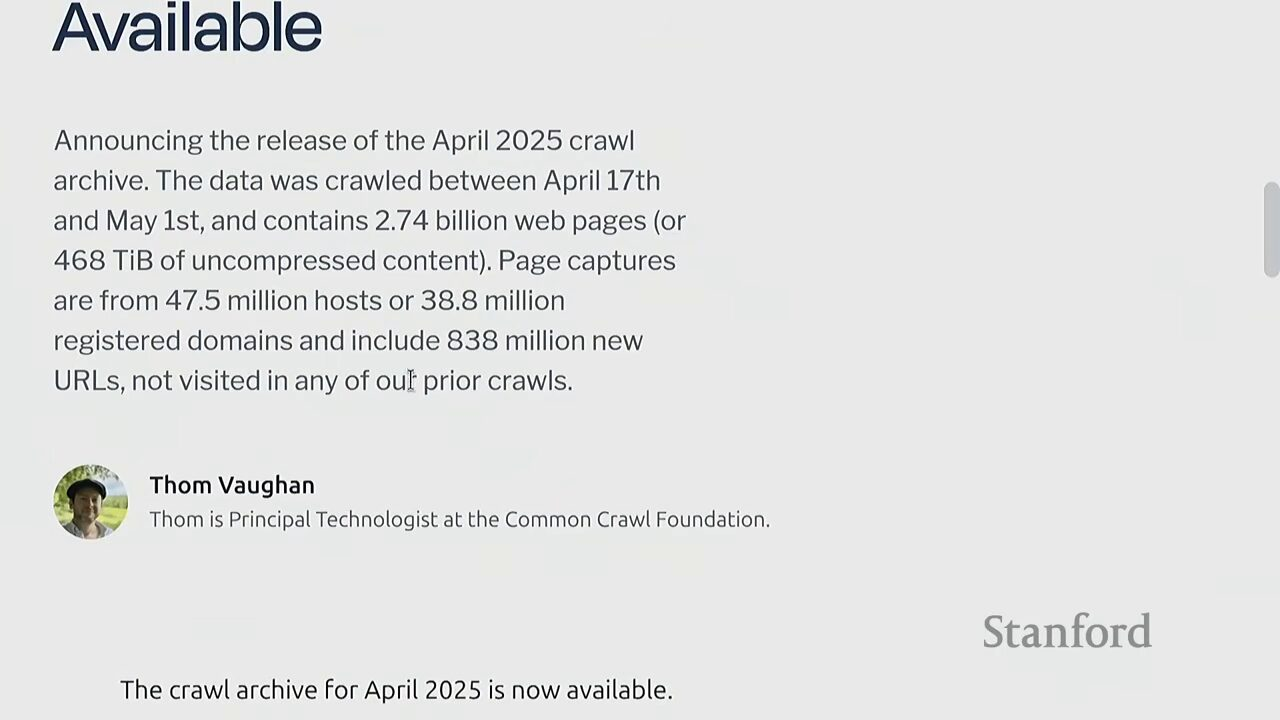
\includegraphics[width=0.95\textwidth]{figures/fig_07_cc_stats.jpg}
\caption{Common Crawl 规模：单个月级快照约 27 亿页面\protect\footnotemark}
\end{figure}
\footnotetext{视频画面时间区间：00:14:30--00:15:15。}

当有人说"语言模型是在互联网上训练的"，你应该追问：\textbf{具体是互联网的哪个子集？}Common Crawl 或许是对"互联网"最接近的学术近似。它成立于 2007 年，每月做一次完整网页爬取，17 年来积累了约 100 多个爬取快照。

\begin{itemize}
\item \textbf{成本}：爬取本身相对于语言模型训练并不算贵——租一批 AWS 机器，两周内能搞定一次。
\item \textbf{规模}：单次月级快照约 \textbf{27 亿页面}。不同快照间有重叠，但 CC 有意识地做多样性尝试。
\item \textbf{内容过滤}：默认非常宽松，含有大量冒犯性/有害内容（因为"是否冒犯"本身是个高层语义判断）。可能有针对明显违法站点的黑名单，但细节不明。
\end{itemize}

\subsection{爬虫是怎么工作的}

\begin{figure}[H]
\centering
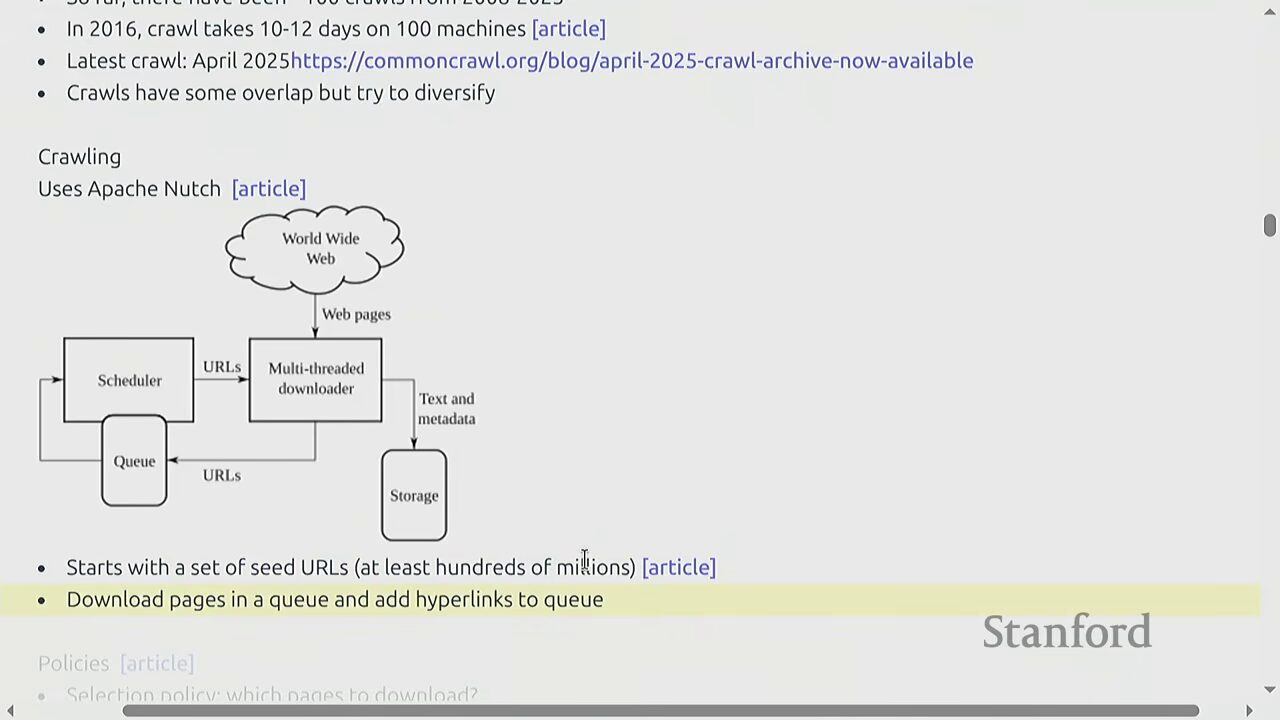
\includegraphics[width=0.95\textwidth]{figures/fig_08_crawl_arch.jpg}
\caption{爬虫架构：从海量 seed URL 出发，维护爬取前沿，多机并行 BFS\protect\footnotemark}
\end{figure}
\footnotetext{视频画面时间区间：00:15:30--00:16:15。}

Common Crawl 用一个开源爬虫库，核心机制是对整个 Web 做 \textbf{广度优先搜索（BFS）}：

\begin{enumerate}
\item \textbf{Seed URLs}：不是从一个网站出发，而是从\textbf{数亿个}种子 URL 开始（这远比想象的多）。
\item \textbf{爬取前沿（crawl frontier）}：维护一个待爬取 URL 的队列。
\item \textbf{并行抓取}：一批机器不断从 frontier 取 URL 去 fetch。
\end{enumerate}

\begin{tcolorbox}[enhanced, colback=blue!5!white, colframe=blue!75!black, sharp corners, title=\textbf{爬虫要处理的工程问题}]
\begin{itemize}
\item \textbf{礼貌性}：尊重 \texttt{robots.txt}，不能压垮目标服务器。
\item \textbf{调度}：哪些页面先爬？已爬过的何时重访？变化快的站点爬得频繁些。
\item \textbf{URL 去重}：URL 是动态的，同一个内容可能有多个超长 URL 指向它，造成大量重复。
\item \textbf{覆盖不全}：CC 有意保持"礼貌"，\textbf{并非}要爬遍整个互联网——甚至不是所有 Wikipedia 文章都在 CC 里。
\end{itemize}
\end{tcolorbox}

\subsection{WARC 与 WET：原始响应 vs. 提取文本}

\begin{figure}[H]
\centering
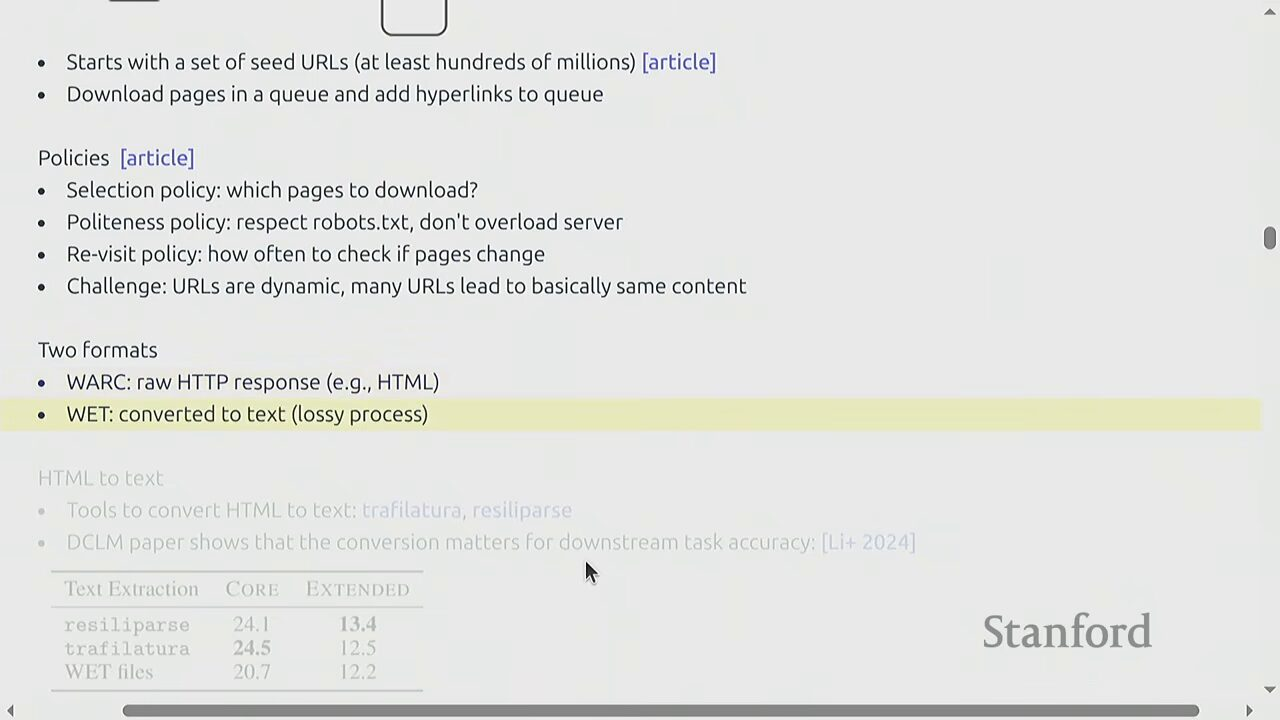
\includegraphics[width=0.95\textwidth]{figures/fig_09_warc_wet.jpg}
\caption{Common Crawl 的两种产物：WARC（原始 HTTP/HTML）与 WET（提取后的纯文本）\protect\footnotemark}
\end{figure}
\footnotetext{视频画面时间区间：00:16:30--00:17:15。}

Common Crawl 对每次爬取提供两种格式：

\begin{itemize}
\item \textbf{WARC（Web ARChive）}：原始 HTTP 响应，对网页来说通常就是 HTML。这是"最原始"的形式。
\item \textbf{WET}：从 HTML 提取出的纯文本。这一步是\textbf{有损}的——HTML 到文本的转换必然丢失信息。
\end{itemize}

\begin{importantbox}{HTML$\to$文本的工具选择，影响巨大}
DataComp 论文做过消融：用 Common Crawl 自带的 WET 文件 vs. 自己用 \texttt{trafilatura}（一个 HTML 解析库）从 WARC 重新提取文本，后者在下游任务上能\textbf{高出整整 4 个点}。这说明低层的文本提取细节直接决定数据质量。Assignment 里会让你亲手尝试不同的 HTML$\to$文本工具。

更激进的是，Nemotron-CC 后来发现 \texttt{justext}（另一个工具）保留的 token 数比 trafilatura 还多——当你既要质量又要量时，这种细微差别就变得关键。
\end{importantbox}

\subsection{robots.txt 与抓取伦理}

\begin{figure}[H]
\centering
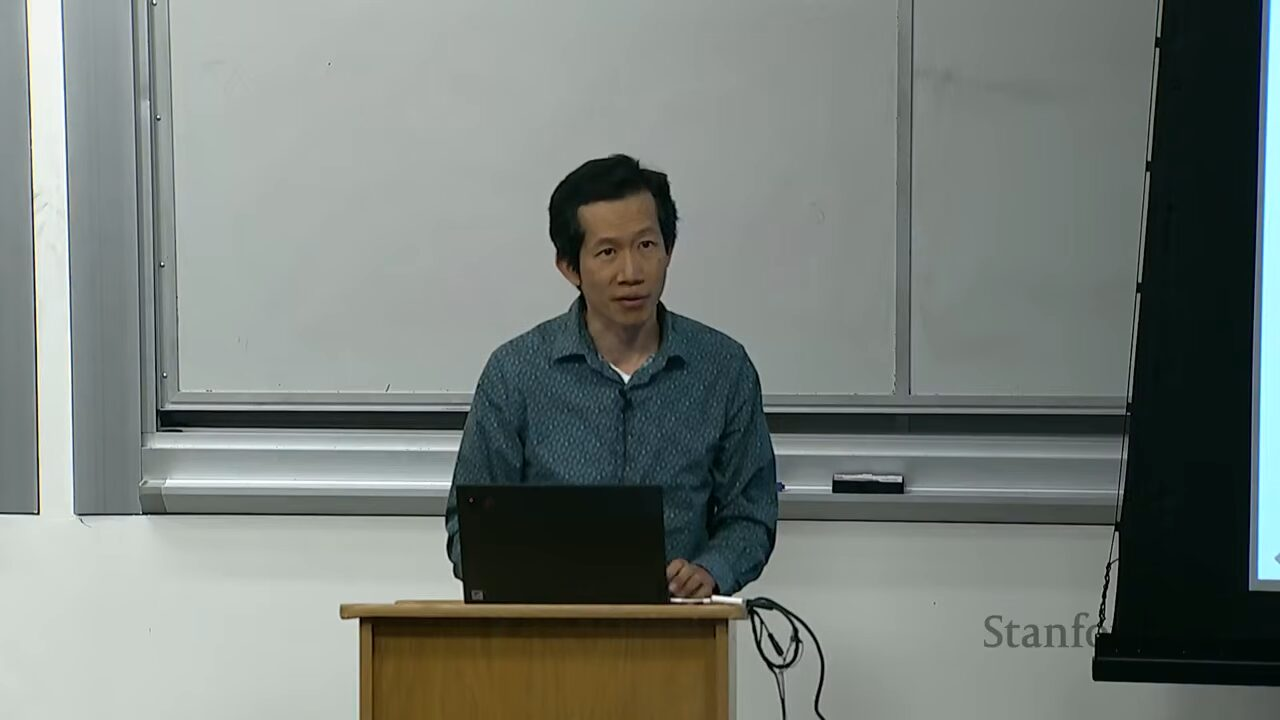
\includegraphics[width=0.92\textwidth]{figures/fig_10_robots.jpg}
\caption{robots.txt：网站声明允许哪些爬虫、禁止哪些路径\protect\footnotemark}
\end{figure}
\footnotetext{视频画面时间区间：00:18:30--00:19:30。}

网站可以在根目录放一个 \texttt{robots.txt}，声明允许哪些爬虫、禁止爬哪些路径。例如 \texttt{nytimes.com} 的 robots.txt 对 Googlebot 有一大堆 disallow 规则；而你会发现\textbf{几乎所有前沿模型厂商都有自己的爬虫}——因为 Common Crawl 的覆盖其实相当稀疏，互联网太大，要拿到新鲜高质量数据非得自己爬不可。

\begin{warningbox}{robots.txt 不是法律}
robots.txt 只是一种\textbf{指导}（guidance），没有正式机制强制执行。可能有不守规矩的爬虫无视它。一个网站即使声明了不想被收录，也无法保证真的不被爬。这是当前数据生态的一个灰色地带。
\end{warningbox}

\section{过滤 Common Crawl 的两条路线}

Common Crawl 很大，但正如第一堂课展示的，随机采样它的内容基本是垃圾。于是出现了大量过滤方案，核心分化为\textbf{两条哲学路线}。

\subsection{CCNet（Meta）：基于模型的"像 Wikipedia"过滤}

\begin{figure}[H]
\centering
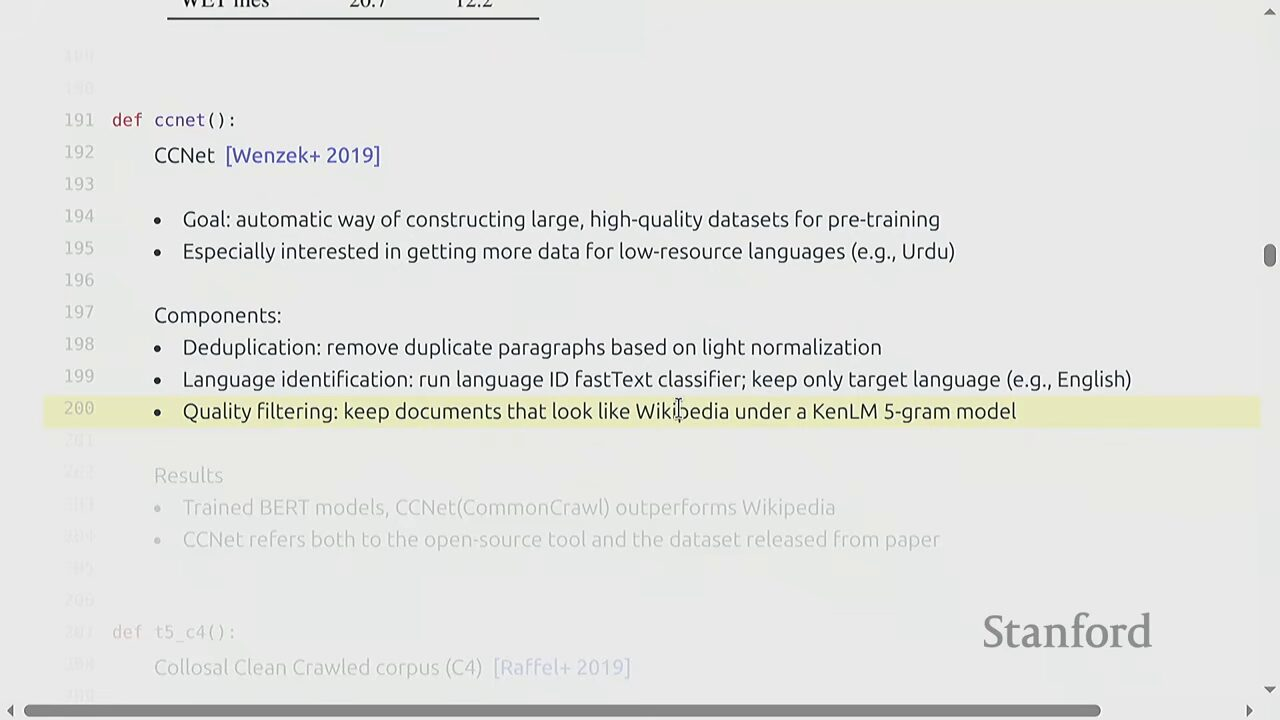
\includegraphics[width=0.92\textwidth]{figures/fig_11_ccnet.jpg}
\caption{CCNet：用 Wikipedia 训练的五元模型给文档打分\protect\footnotemark}
\end{figure}
\footnotetext{视频画面时间区间：00:23:00--00:23:45。}

CCNet 是 Meta 早期（用于训练 RoBERTa 等）的工作，目标是构造一个通用流程，把 Common Crawl 转成高质量数据集，特别关注多语言覆盖。它的处理管线是：

\begin{enumerate}
\item \textbf{语言识别}：用一个线性分类器判定每篇文档的语言，只保留目标语言（英语、德语等）。
\item \textbf{去重}：移除重复文档。
\item \textbf{质量过滤（关键）}：用 Wikipedia 文本训练一个 \textbf{5-gram 语言模型}，用它给每篇文档打分。\emph{分数高意味着这篇文档"长得像 Wikipedia"}。
\end{enumerate}

\begin{knowledgebox}{Wikipedia 作为质量代理}
CCNet 把 Wikipedia 当作高质量数据的代理（surrogate）：分数高 = 像 Wikipedia = 高质量。但这恰恰继承了 Wikipedia 的盲区——那些不像百科条目却依然优质的内容（小说、对话、代码注释）会被打低分而流失。这种"代理偏差"是基于模型过滤的固有代价。
\end{knowledgebox}

\subsection{C4（Google）：纯启发式规则}

\begin{figure}[H]
\centering
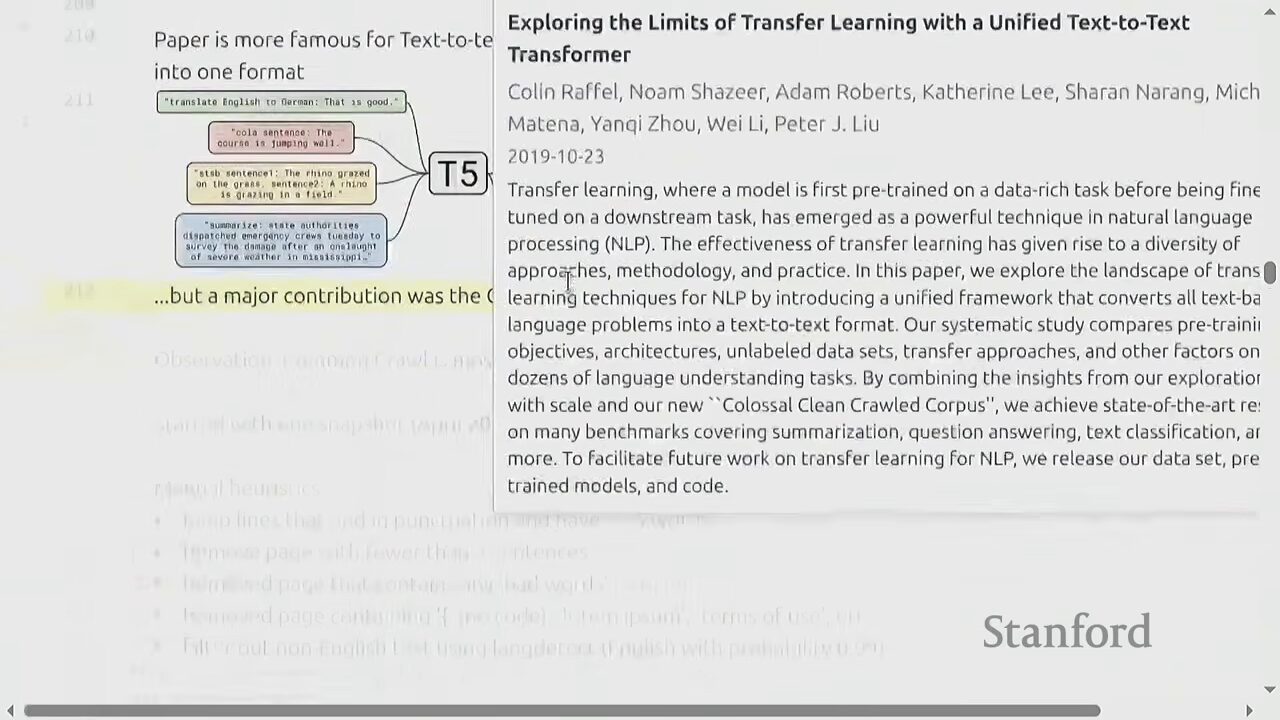
\includegraphics[width=0.95\textwidth]{figures/fig_12_c4.jpg}
\caption{C4（Colossal Clean Crawled Corpus）：完全用手工规则清洗\protect\footnotemark}
\end{figure}
\footnotetext{视频画面时间区间：00:24:15--00:25:00。}

C4 来自 Colm Rafferty 那篇以 T5 模型闻名的论文（但 C4 数据集本身是主要贡献）。从 1.4T tokens 的单个 CC 快照出发，\textbf{完全不用模型}，只用一堆手工规则：

\begin{itemize}
\item 只保留以标点结尾的行。
\item 删除少于 3 个句子的页面。
\item 删除含"脏词"的页面（有一个 bad words 列表）。
\item 删除花括号 \texttt{\{...\}} 内容（这会删掉大量代码，但 Python 可能侥幸保留）。
\item 删除样板文字（boilerplate）。
\item 只保留英语。
\end{itemize}

\begin{importantbox}{两条路线的互补性与权衡}
\begin{itemize}
\item \textbf{基于模型（CCNet）}：只能找到"像你提供的正例"的内容。当你想要\emph{广泛覆盖}时，很难为每种好内容都准备代表性正例——这正是你试图策展的难题本身。
\item \textbf{基于规则（C4）}：能保留不像 Wikipedia 但结构良好的句子；但也会放进"语法正确但内容垃圾"的句子（比如精心写的垃圾营销文案）。
\end{itemize}
两者是\textbf{互补}的：一个偏精确率，一个偏召回率。C4 里还能看到大量专利和新闻——这些都是规则的副产品。
\end{importantbox}

\subsection{WebText-like：CC 的覆盖其实很有限}

C4 论文还做了一个 WebText-like 数据集：拿 OpenWebText 的 Reddit（karma $> 3$）链接去 Common Crawl 的 12 个 dump 里找。即便用了这么多 dump，也只得到 \textbf{17 GB 文本}——而原始 WebText 是 40 GB。这说明 Common Crawl 的覆盖\textbf{相当不完整}：很多 Reddit 高赞链接指向的页面根本没被 CC 抓到。

\section{GPT-3 时代：质量分类器的兴起}

\subsection{GPT-3 数据集}

\begin{figure}[H]
\centering
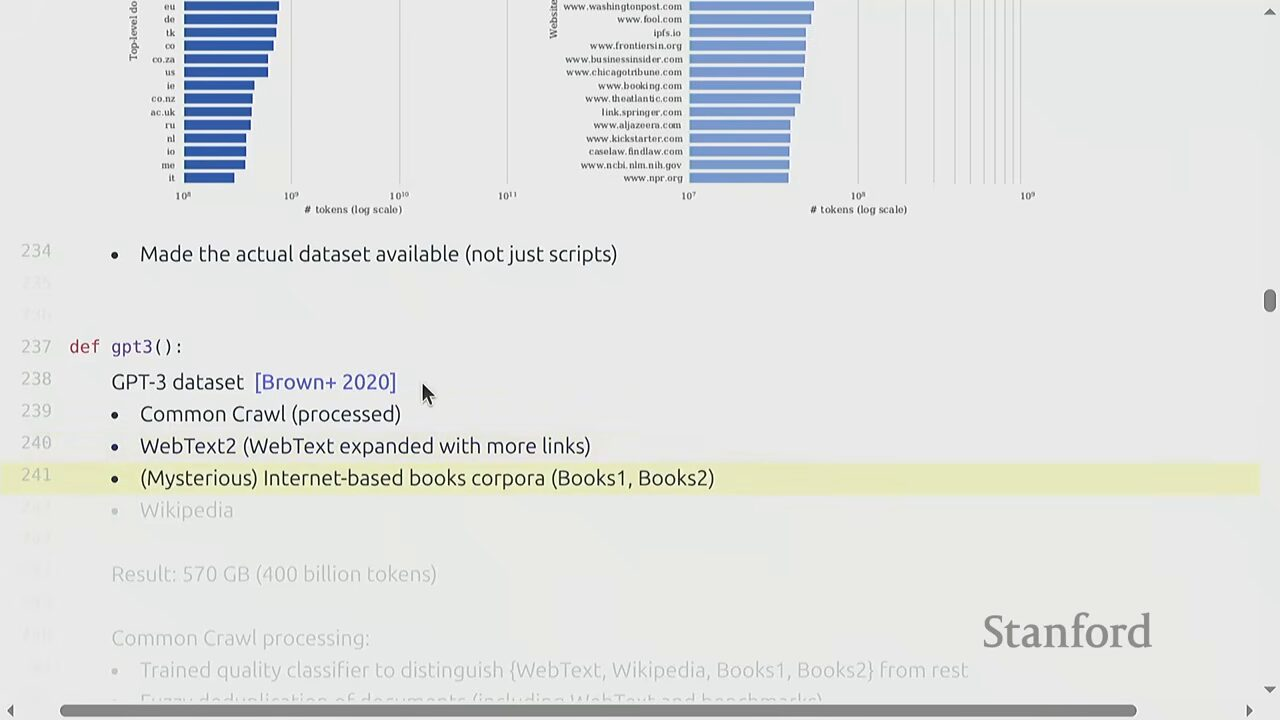
\includegraphics[width=0.92\textwidth]{figures/fig_13_gpt3.jpg}
\caption{GPT-3 的数据组成与质量分类器筛选流程\protect\footnotemark}
\end{figure}
\footnotetext{视频画面时间区间：00:28:00--00:28:45。}

GPT-3 的数据集约 \textbf{400B tokens}（按今天的标准很小，当时很惊人），由四部分组成：处理过的 Common Crawl、WebText2（GPT-2 那套思路）、神秘的 Books1/Books2、以及 Wikipedia。

关键创新是 \textbf{质量分类器}：

\begin{enumerate}
\item 把 WebText、Wikipedia、Books 标为\textbf{正例}（高质量）。
\item 从 Common Crawl 随机采样作为\textbf{负例}。
\item 训一个二分类器，然后用它在更大的 Common Crawl 池子里\emph{捞更多像正例的数据}。
\end{enumerate}

\begin{knowledgebox}{质量分类器的范式}
这是数据工程的里程碑：\textbf{先定义"什么是好"，再去大池子里找更多"好"}。后续几乎所有模型都用了这个范式。它的灵活性在于——你可以把"好"定义成任意东西：像 Wikipedia、像指令数据、像数学推导……正例的选择决定了你能捞出什么。
\end{knowledgebox}

\subsection{The Pile（EleutherAI，2020）：22 个策展领域}

\begin{figure}[H]
\centering
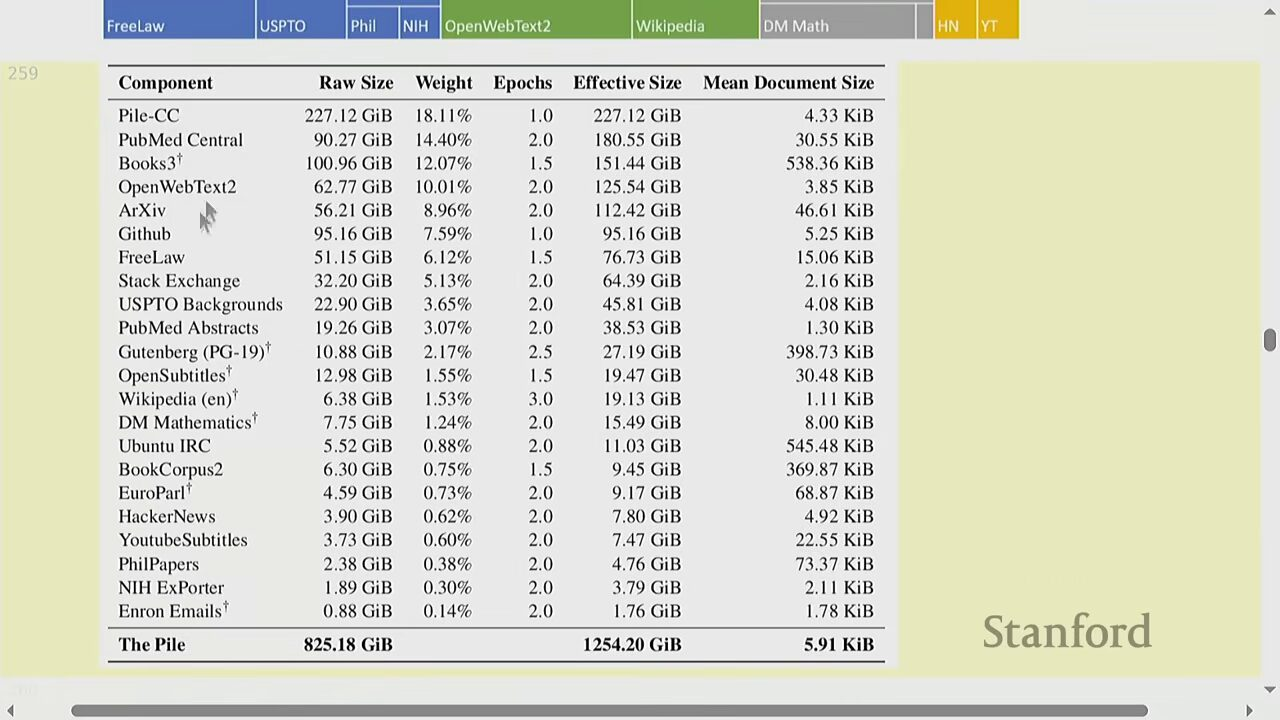
\includegraphics[width=0.95\textwidth]{figures/fig_14_pile.jpg}
\caption{The Pile：EleutherAI 社区驱动的 22 个高质量数据领域\protect\footnotemark}
\end{figure}
\footnotetext{视频画面时间区间：00:30:00--00:30:45。}

GPT-3 的封闭引发了 EleutherAI 的诞生——一个去中心化、Discord 驱动的志愿者组织，目标是复现开源语言模型。他们策展了 \textbf{The Pile}，包含 22 个"大家觉得高质量"的领域：Common Crawl、OpenWebText、Stack Exchange、Wikipedia、arXiv 等等。这个数据集比 GPT-3 训练用的还大。

The Pile 里几个有意思的组件值得展开，因为它们揭示了"专门处理某类数据"的价值：

\begin{tcolorbox}[enhanced, colback=blue!5!white, colframe=blue!75!black, sharp corners, title=\textbf{The Pile 里的特色数据源}]
\begin{description}
\item[PubMed Central] 大量开放获取的医学论文（NIH 资助的工作必须开放）。在 AI 领域我们习惯了 arXiv，但其他学科并非如此。
\item[arXiv] 预印本服务器。
\item[Enron 邮件] 这是个\textbf{老数据集}，来自 Enron 公司倒闭后的法庭传票。\textbf{为什么要在里面？}因为真实的邮件数据集极其稀缺（邮件是隐私），这是我们能拿到的最好替代——虽然显然带有这家倒闭公司的偏见。
\item[Project Gutenberg] 详见下节。
\end{description}
\end{tcolorbox}

\section{专门数据源深入}

\subsection{Project Gutenberg 与 Books}

Project Gutenberg 是一个老牌项目，主要是英语公共领域书籍（出版满 75 年、版权过期），现有约 \textbf{75,000 本}。最大的卖点是\textbf{版权清晰}——可以自由使用。\textbf{PG19} 是基于它的一个 benchmark，专门测长上下文能力——因为书的上下文远比新闻或论文长。

\textbf{Books3} 则截然不同：它从一个\textbf{影子图书馆}（shadow library）抓取了大量名家著作，包含大量仍在版权期的书。它已被因版权侵权下架，并且\textbf{Meta 因为在 LibGen 上训练模型而卷入重大诉讼}。

\begin{warningbox}{影子图书馆（Shadow Libraries）}
这些图书馆\textbf{无视版权、绕过付费墙}，本质上是非法的。LibGen 有约 400 万本书（对比 Gutenberg 的 7.5 万）。尽管有大量禁令和诉讼，它们通常通过把服务器放在不同国家来规避管制。支持者认为"该免费的就该免费"，法律显然不同意。LLaMA 训练用 Books3 惹的麻烦，就是这个问题的现实后果。
\end{warningbox}

\subsection{Stack Exchange：天然的问答对}

\begin{figure}[H]
\centering
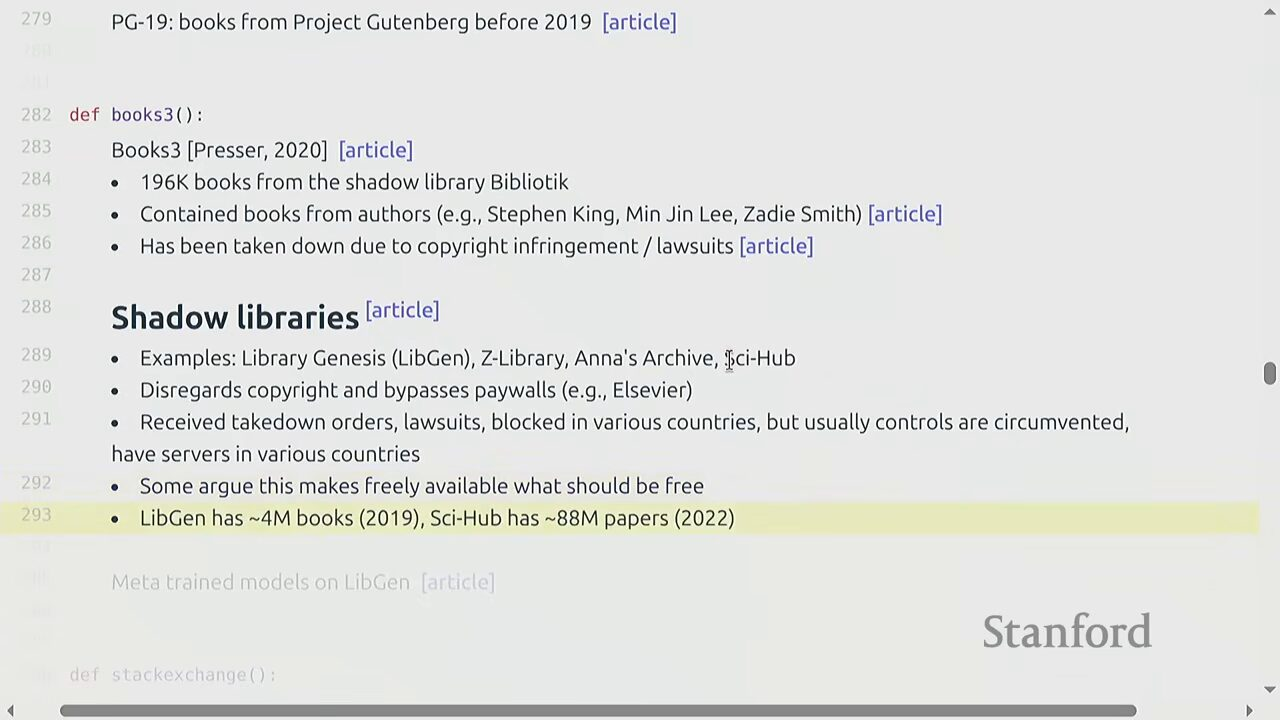
\includegraphics[width=0.92\textwidth]{figures/fig_15_stackexchange.jpg}
\caption{Stack Exchange：问答对格式天然贴近指令跟随场景\protect\footnotemark}
\end{figure}
\footnotetext{视频画面时间区间：00:36:00--00:36:45。}

Stack Exchange 是一组网站（最出名的是 Stack Overflow，还有数学、文学等），有声誉系统和徽章激励参与。它的数据有几个独特性质：

\begin{itemize}
\item \textbf{天然 QA 格式}：问题 + 回答，这正是用户和聊天机器人交互的形式——所以\emph{预训练数据里有相当一部分已经"长得像"指令跟随数据}，pre-training 和 post-training 的界限因此模糊。
\item \textbf{丰富的元数据}：评论、投票分数都可以用来做质量过滤。
\item \textbf{数据 dump 开放}：非商用免费，商用需购买许可。注意 2023 年前后 Stack Exchange、Reddit 等都意识到"别人白嫖我们的数据训练模型赚钱"，纷纷收紧了政策。
\end{itemize}

\subsection{GitHub：代码来源与处理挑战}

\begin{figure}[H]
\centering
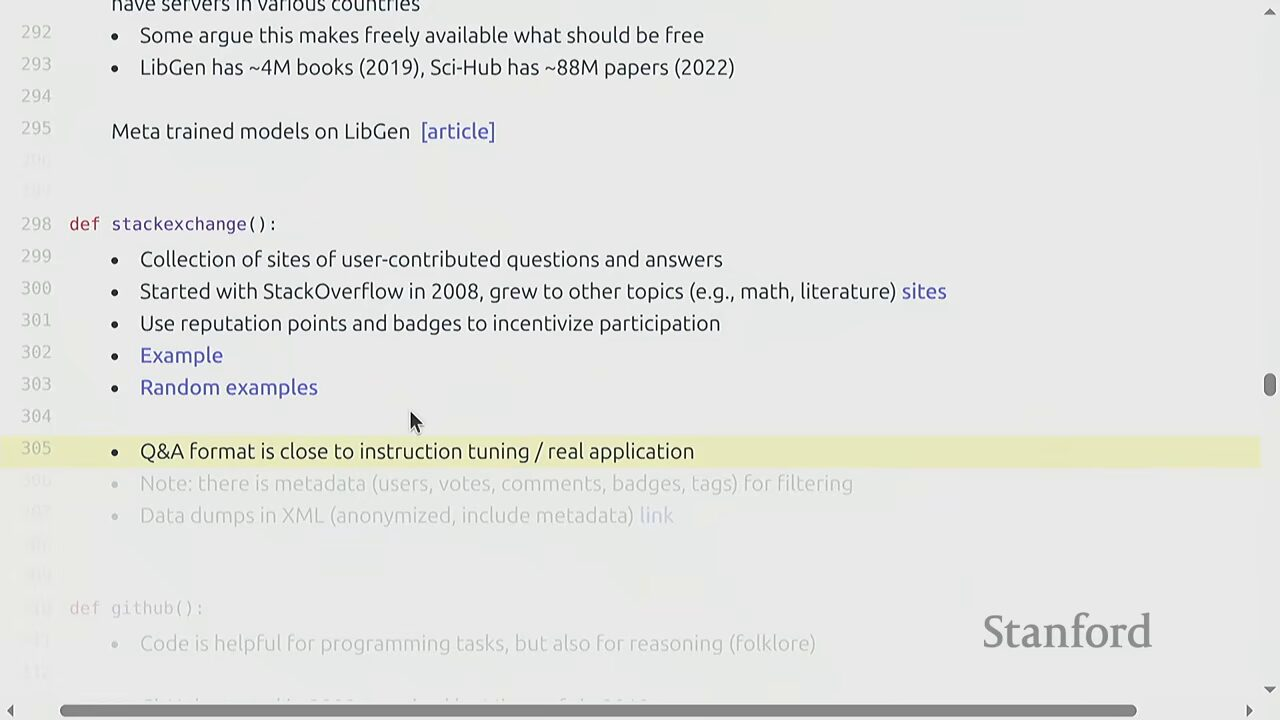
\includegraphics[width=0.92\textwidth]{figures/fig_16_github.jpg}
\caption{GitHub：2800 万公开仓库，但仓库 $\neq$ 可训练 tokens\protect\footnotemark}
\end{figure}
\footnotetext{视频画面时间区间：00:38:00--00:38:45。}

GitHub 有约 \textbf{2800 万公开仓库}，是代码数据的主要来源。代码不仅对编程能力有用，还被认为有助于推理能力（虽然 Percy 坦言没有严格论文支持这点）。但处理 GitHub 远比想象复杂：

\begin{tcolorbox}[enhanced, colback=blue!5!white, colframe=blue!75!black, sharp corners, title=\textbf{从 GitHub 到可训练代码：三步抽象}]
\begin{enumerate}
\item \textbf{Live service}：你每天访问的 GitHub 网站。
\item \textbf{Raw dump}：\texttt{GitHub Archive} 是所有 GitHub 事件的快照，可用 Google BigQuery 查询。
\item \textbf{处理后的数据集}：例如 \textbf{The Stack}，从 GitHub Archive 拿到仓库名，git clone 了 137M 个仓库，只保留宽松许可证的，去重后得到 \textbf{3.1 TB 代码}。
\end{enumerate}
\end{tcolorbox}

\begin{importantbox}{"我用了 GitHub 训练"——追问细节}
当有人说"我在 GitHub 上训练"，你应该追问：\textbf{到底用了哪个抽象层级？经过了什么预处理？}仓库是目录，里面有代码也有非代码（issues、commit 历史），还有大量重复。代码的一个好处是\textbf{许可证通常比网页清晰}（虽然不总是）——这是相对网页数据的一个优势。
\end{importantbox}

\section{2021--2024：数据工程的成熟期}

\subsection{MassiveText（DeepMind，2021）：手工规则 + 安全搜索}

\begin{figure}[H]
\centering
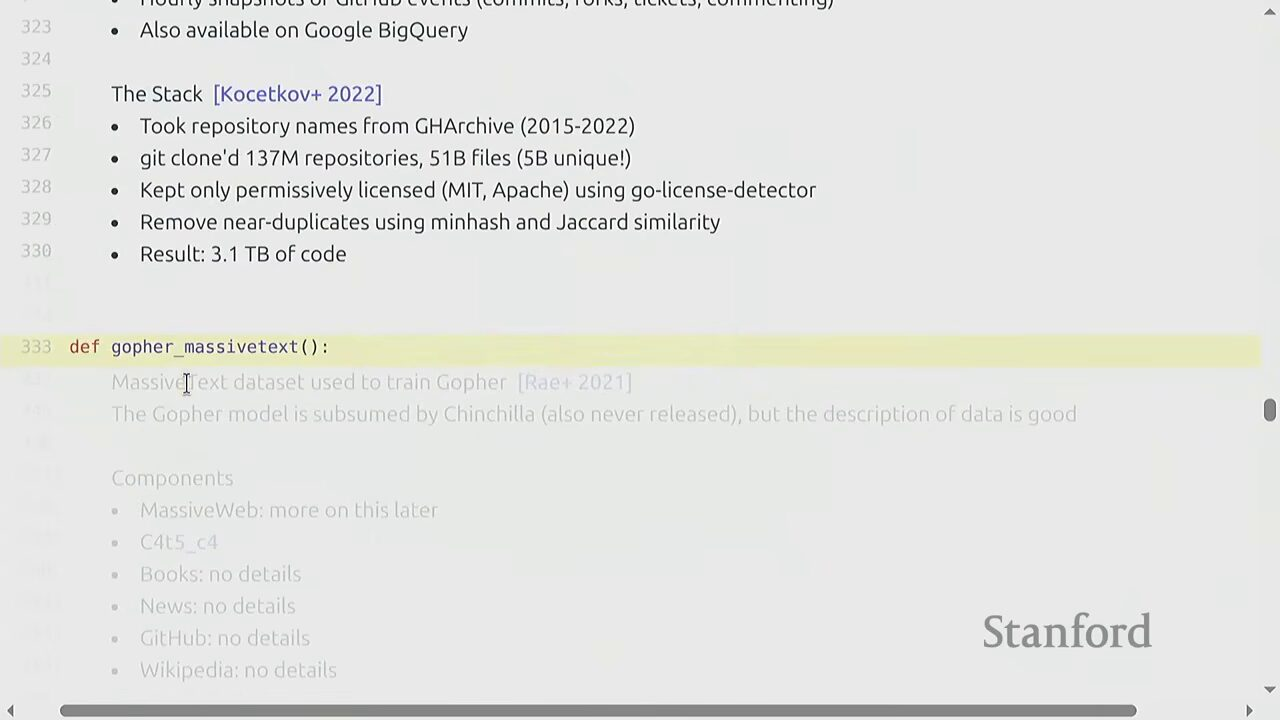
\includegraphics[width=0.92\textwidth]{figures/fig_17_massivetext.jpg}
\caption{MassiveText（Gopher）：包含 MassiveWeb、C4、书籍、新闻、GitHub、Wikipedia\protect\footnotemark}
\end{figure}
\footnotetext{视频画面时间区间：00:42:00--00:42:45。}

DeepMind 的第一个大模型 Gopher 训练在 \textbf{MassiveText} 上（Gopher 本身不太行，但数据集论文描述得很好）。数据集约 \textbf{10 TB 文本}（估算 4--5T tokens），包含 MassiveWeb、C4、书籍、新闻、GitHub、Wikipedia（除 MassiveWeb 外都没给处理细节，不可复现）。

\textbf{MassiveWeb} 的过滤策略：保留英语 + 手工规则（assignment 里你会实现的"Gopher rules"，比如 80\% 的词必须含至少一个字母字符）+ Google Safe Search 做\textbf{毒性过滤}。

\begin{knowledgebox}{为什么当时坚持用手工规则？}
2021 年坚持用手工规则而非模型过滤，有两个理由：\textbf{(1)} 当时能跑的模型太弱，弱模型不理解页面，反而引入糟糕的偏见；\textbf{(2)} 担心模型过滤会\emph{系统性排除边缘群体}的内容——因为那些内容"不像 Wikipedia"。但这个立场后来\textbf{完全反转}：今天大家都在用模型过滤，因为收益太大了。这是一个值得记住的范式转向。
\end{knowledgebox}

\subsection{LLaMA（Meta，2022）：被引用的页面}

\begin{figure}[H]
\centering
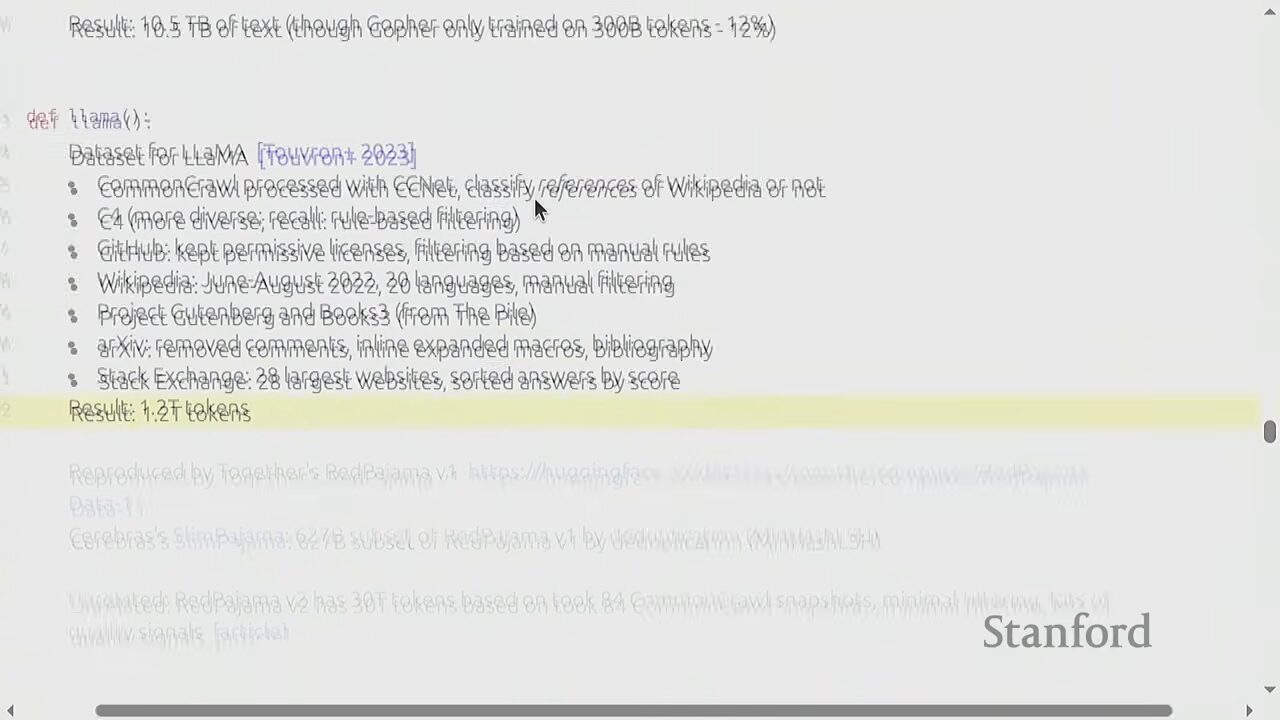
\includegraphics[width=0.92\textwidth]{figures/fig_18_llama.jpg}
\caption{LLaMA 数据集：CCNet 处理的 CC + C4 + GitHub + Wikipedia + Gutenberg + arXiv + Stack Exchange\protect\footnotemark}
\end{figure}
\footnotetext{视频画面时间区间：00:45:30--00:46:15。}

LLaMA 的数据约 \textbf{1.2T tokens}，包含 CCNet 处理的 Common Crawl、C4、GitHub（宽松许可证 + 手工规则过滤）、Wikipedia、Project Gutenberg、Books3（惹麻烦的那个）、arXiv、Stack Exchange。

\begin{importantbox}{分类器设计的一个精妙差别}
GPT-3 的分类器问的是：\textbf{"这篇文档像不像 Wikipedia 页面？"}\\
LLaMA 的分类器问的是：\textbf{"这篇文档像不像被 Wikipedia \emph{引用}的页面？"}

差别巨大！Wikipedia 会引用高质量外部页面，但这些页面本身可能完全不像百科条目（比如个人博客的深度技术分析）。借由这种\emph{引用结构}，LLaMA 能捞到"高质量但不像 Wikipedia"的内容。这又是 WebText 那个"用链接结构定位质量"思想的回响。
\end{importantbox}

LLaMA 没发布数据集，社区复刻成 \textbf{RedPajama}（有处理代码和数据）。Cerebras 进一步去重得到 627B 的子集。\textbf{RedPajama v2} 是另一个东西——拿 CC 快照产出 \textbf{30T tokens} 并附带各种质量信号，供研究如何按信号过滤。

\subsection{RefinedWeb / FineWeb：只用网页够不够}

\begin{figure}[H]
\centering
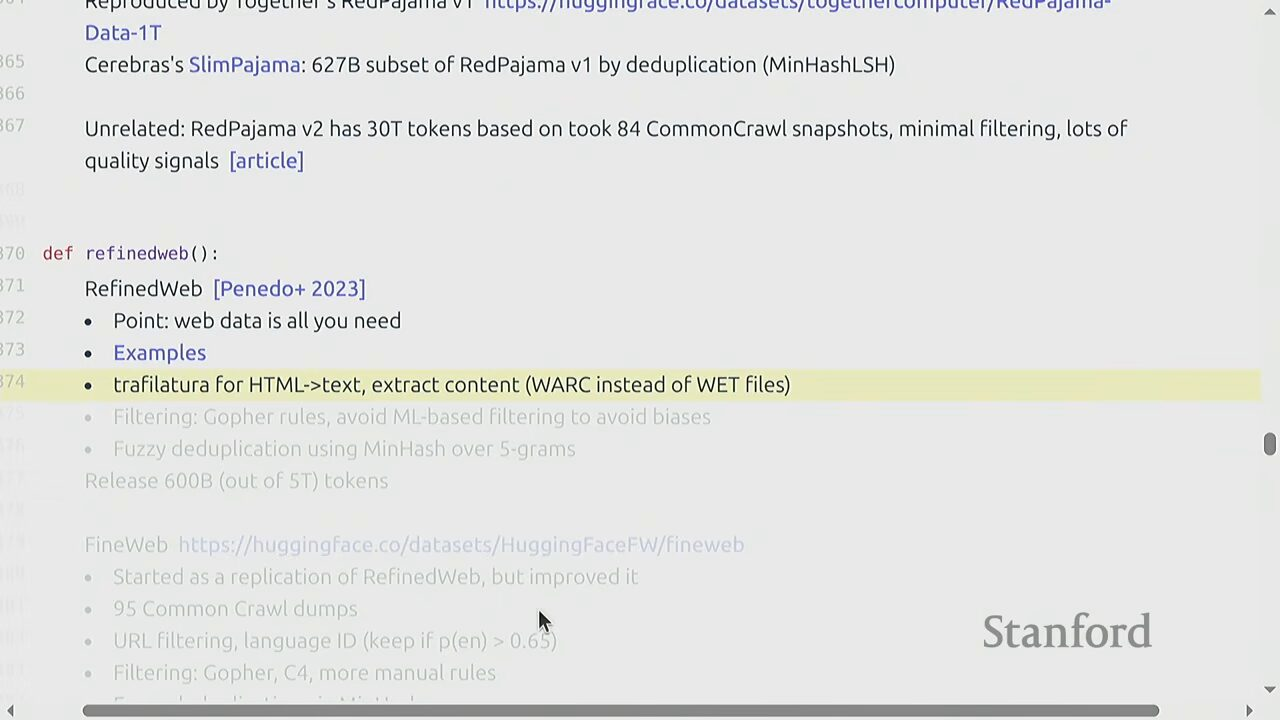
\includegraphics[width=0.92\textwidth]{figures/fig_19_fineweb.jpg}
\caption{RefinedWeb 的论点：把网页数据过滤好，就够了\protect\footnotemark}
\end{figure}
\footnotetext{视频画面时间区间：00:47:30--00:48:15。}

RefinedWeb 的论点是挑衅性的：\textbf{回忆 The Pile，里面有网页 + 一堆专门来源。但如果把网页过滤得足够好，也许网页就够了}——毕竟从某种意义上，互联网上什么都有，只要能通过电脑访问到的东西都在网上。

它的做法：用 \texttt{trafilatura} 提取内容（比 WET 好）、Gopher rules、\textbf{刻意避免 ML 过滤}（怕偏见）、做模糊去重。结果是 5T tokens 的数据集（只发布 600B）。\textbf{FineWeb}（Hugging Face）是 RefinedWeb 的复刻+改进：用所有 CC dump、手工规则过滤、去重、基本匿名化，得到 \textbf{15T tokens}。

\begin{practicebox}{FineWeb 的定位}
把 FineWeb 理解为一个\textbf{轻度过滤}的数据集——在上面你还可以进一步做基于模型的过滤。它是"Common Crawl 太难处理"和"想要干净起点"之间的一个甜蜜点。
\end{practicebox}

\subsection{DOLMA（AI2 OLMo，2023）：多源组合}

\begin{figure}[H]
\centering
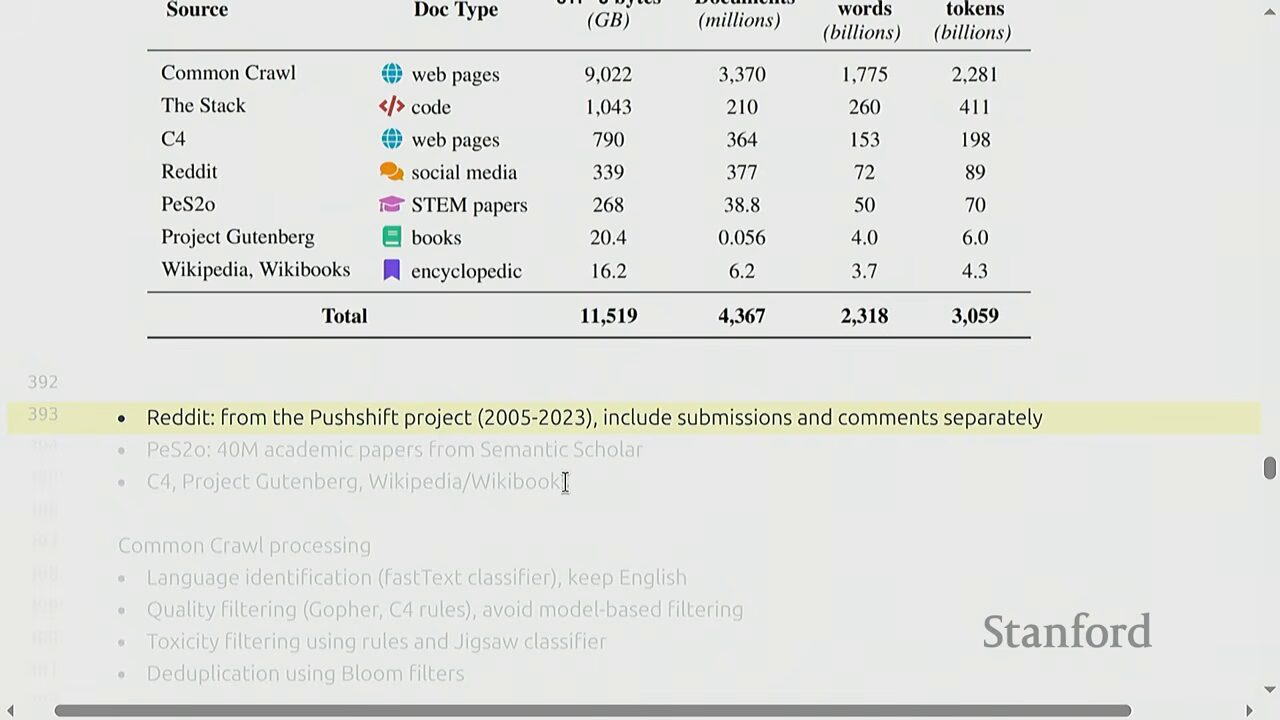
\includegraphics[width=0.92\textwidth]{figures/fig_20_dolma.jpg}
\caption{DOLMA：AI2 为 OLMo 构建的多源数据组合\protect\footnotemark}
\end{figure}
\footnotetext{视频画面时间区间：00:49:45--00:50:30。}

AI2 的 OLMo 初始模型训练在 \textbf{DOLMA} 上：Common Crawl、The Stack（代码）、C4、Reddit、Semantic Scholar（4000 万学术论文）、Project Gutenberg、Wikipedia。Common Crawl 的处理是标准的：语言识别保留英语 + 质量过滤（初版刻意\emph{避免}模型过滤）+ 毒性分类器 + 去重，得到 \textbf{3T tokens}。

注意 Reddit 那部分来自一个已不存在的项目，把提交和评论分开存储（丢失了线程结构）——2023 年前后 Reddit 收紧数据政策，这类项目大多停摆。

\subsection{DataComp / DCLM（2024）：把数据集做成竞赛}

\begin{figure}[H]
\centering
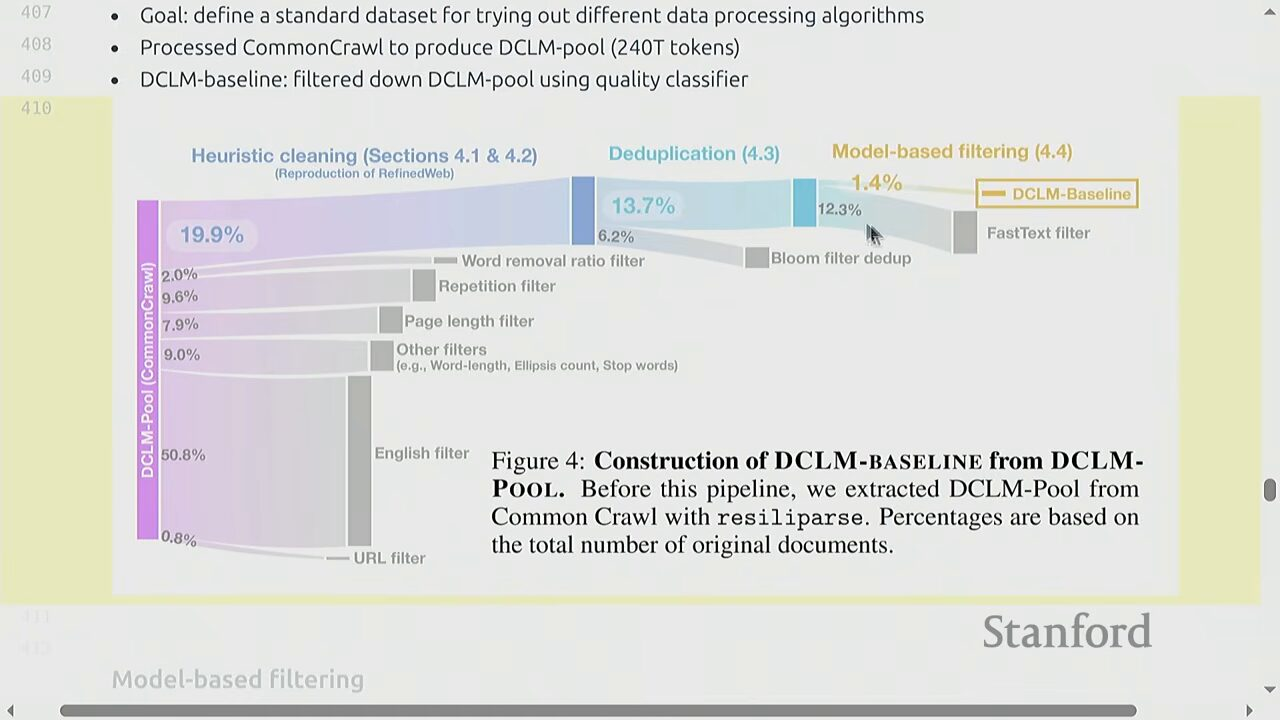
\includegraphics[width=0.95\textwidth]{figures/fig_21_datacomp.jpg}
\caption{DataComp/DCLM：从 240T token 池子筛选至 3.8T 的 baseline\protect\footnotemark}
\end{figure}
\footnotetext{视频画面时间区间：00:52:00--00:52:45。}

DataComp 是多组织合作，核心想法是\textbf{把数据集创建变成一个标准化的竞赛}：定义公共的数据池和评测协议，让大家比拼数据处理算法。他们处理所有 CC dump 产出 \textbf{DCLM pool（240T tokens）}——量极大但平均质量低，需要大幅过滤。

\textbf{DCLM baseline} 的过滤非常激进：基础规则过滤 + 一个 fastText 质量分类器，最终只保留池子的 \textbf{约 1.4\%}（240T $\to$ 3.8T）。这个分类器的正例选择很巧妙：

\begin{itemize}
\item \textbf{正例来源 1：OpenHermes}——主要是 GPT-4 生成的指令数据。\emph{用指令数据来策展预训练数据}，不是要直接训指令，而是找"长得像指令"的网页。
\item \textbf{正例来源 2：ELI5}——Reddit 的 "Explain Like I'm Five" 子版块，是用户会问聊天机器人的那种问题。
\item \textbf{负例}：从 RefinedWeb 随机采样（不是低质量，只是没那么精心策展）。
\end{itemize}

\begin{importantbox}{结果与范式转向}
用这个 fastText 分类器，DCLM baseline 在 core 基准（HellaSwag 等）上比 RefinedWeb \textbf{高出 3\%}，比其他方案高 1--2\%。更重要的是：第二个 OLMo 模型也开始在 DCLM baseline 上训练了。\textbf{"我们不用模型、保持无偏"的时代基本结束了}——人们意识到在回路里用模型能显著提升数据质量和 benchmark 分数。这是从 MassiveText 时代到今天的最大转向。
\end{importantbox}

\subsection{Nemotron-CC（Nvidia，2024）：把池子做大}

\begin{figure}[H]
\centering
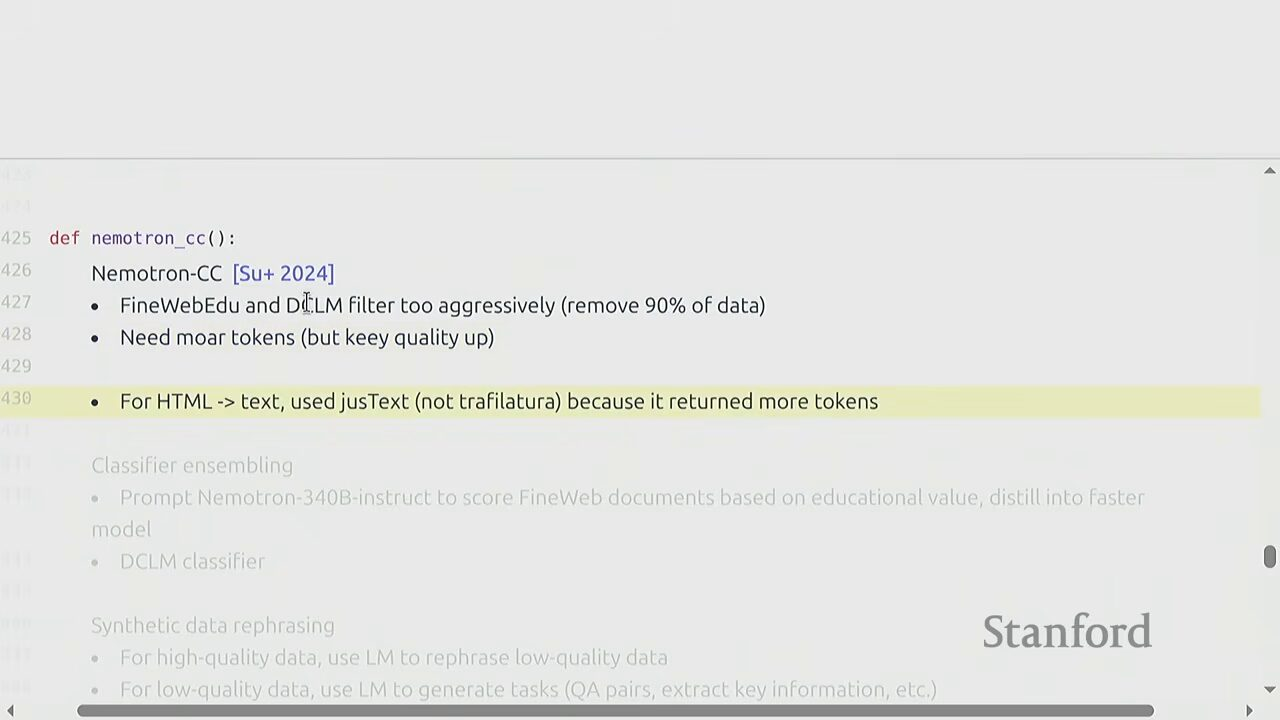
\includegraphics[width=0.92\textwidth]{figures/fig_22_nemotron.jpg}
\caption{Nemotron-CC：教育价值评分 + LM 改写/扩写，从 CC 拿到 6.3T tokens\protect\footnotemark}
\end{figure}
\footnotetext{视频画面时间区间：00:56:00--00:56:45。}

Nvidia 的 Nemotron-CC 针对 DCLM 的一个痛点：\textbf{过滤太狠}。从 240T 砍到 3.8T，要训更大的模型、跑更长的训练，这点数据不够（撑不起 400B 模型的训练 run）。Nemotron 的策略是\textbf{既要质量又要量}：

\begin{tcolorbox}[enhanced, colback=blue!5!white, colframe=blue!75!black, sharp corners, title=\textbf{Nemotron-CC 的关键技术}]
\begin{enumerate}
\item \textbf{HTML$\to$文本重选}：发现 \texttt{justext} 比 \texttt{trafilatura} 保留更多 token——在 token 预算紧张时这个选择很关键。
\item \textbf{教育价值评分}：用他们巨大的 Nemotron 模型给文档打"教育价值"分，蒸馏到一个更快的分类器。同时用 DCLM 分类器。
\item \textbf{分桶采样而非取 top}：把多个分类器的分数分桶，从每个桶采样，确保覆盖不同"质量意见"——不是简单取最高分。
\item \textbf{LM 改写低质量数据}：用大模型把低质量文档\emph{改写}成高质量版本（可能有错，但也许不比训低质量网页更差）。
\item \textbf{LM 扩写高质量数据为任务}：拿一篇 Wikipedia，让大模型生成输入-输出对（问答、摘要、信息抽取）——提前为指令跟随铺路。
\end{enumerate}
\end{tcolorbox}

结果是 \textbf{6.3T tokens}（几乎是 DCLM 的两倍），且平均质量优于 DCLM，并有一个 1T 的高质量子集更好。作为参考：LLaMA 3 训练用了 15T，GPT-3（这里口误，指某最新模型）用了 36T（含多模态）。6.3T 对开源模型已经相当够用，甚至够跑一个 epoch。

\section{数据集演化图谱：一张速查表}

为了把上面这些名字理清楚，下表按时间顺序汇总了主要预训练数据集的关键参数：

\begin{table}[H]
\centering
\small
\begin{tabular}{p{2.3cm}p{2.0cm}p{3.2cm}p{2.0cm}p{3.5cm}}
\toprule
\textbf{数据集} & \textbf{年份} & \textbf{主要来源} & \textbf{规模} & \textbf{过滤哲学} \\
\midrule
BooksCorpus & 2015 & 自出版电子书 & 7K 本 & 无（直接爬取） \\
WebText (GPT-2) & 2019 & Reddit karma$\geq$3 外链 & 40 GB & 社交投票筛选 \\
C4 & 2019 & Common Crawl & $\sim$750 GB & 纯启发式规则 \\
CCNet & 2019 & Common Crawl & 多语言 & Wikipedia 5-gram 模型 \\
GPT-3 数据 & 2020 & CC + WebText2 + Books + Wiki & $\sim$400B tok & 质量分类器（像 Wiki） \\
The Pile & 2020 & 22 个策展领域 & $\sim$825 GB & 社区策展 + 各源专门处理 \\
MassiveText & 2021 & CC + C4 + 书籍 + 代码 + ... & $\sim$10 TB & Gopher rules + SafeSearch \\
LLaMA 数据 & 2022 & CCNet + C4 + GitHub + ... & $\sim$1.2T tok & 分类器（被 Wiki 引用） \\
RefinedWeb & 2023 & 仅 Common Crawl & 5T / 发布 600B & 规则 + 模糊去重（无 ML） \\
FineWeb & 2024 & 所有 CC dump & 15T tok & 手工规则 + 去重 \\
DOLMA & 2023 & CC + Stack + C4 + S2 + ... & 3T tok & 规则 + 毒性分类 + 去重 \\
DCLM baseline & 2024 & Common Crawl & 3.8T tok（池 240T） & fastText 质量分类器 \\
Nemotron-CC & 2024 & Common Crawl & 6.3T tok & 教育评分 + LM 改写/扩写 \\
\bottomrule
\end{tabular}
\caption{主要预训练数据集的演化（2015--2024）。规模单位按原始论文表述。}
\end{table}

\section{版权与合理使用}

\subsection{大部分互联网内容都是版权的}

\begin{figure}[H]
\centering
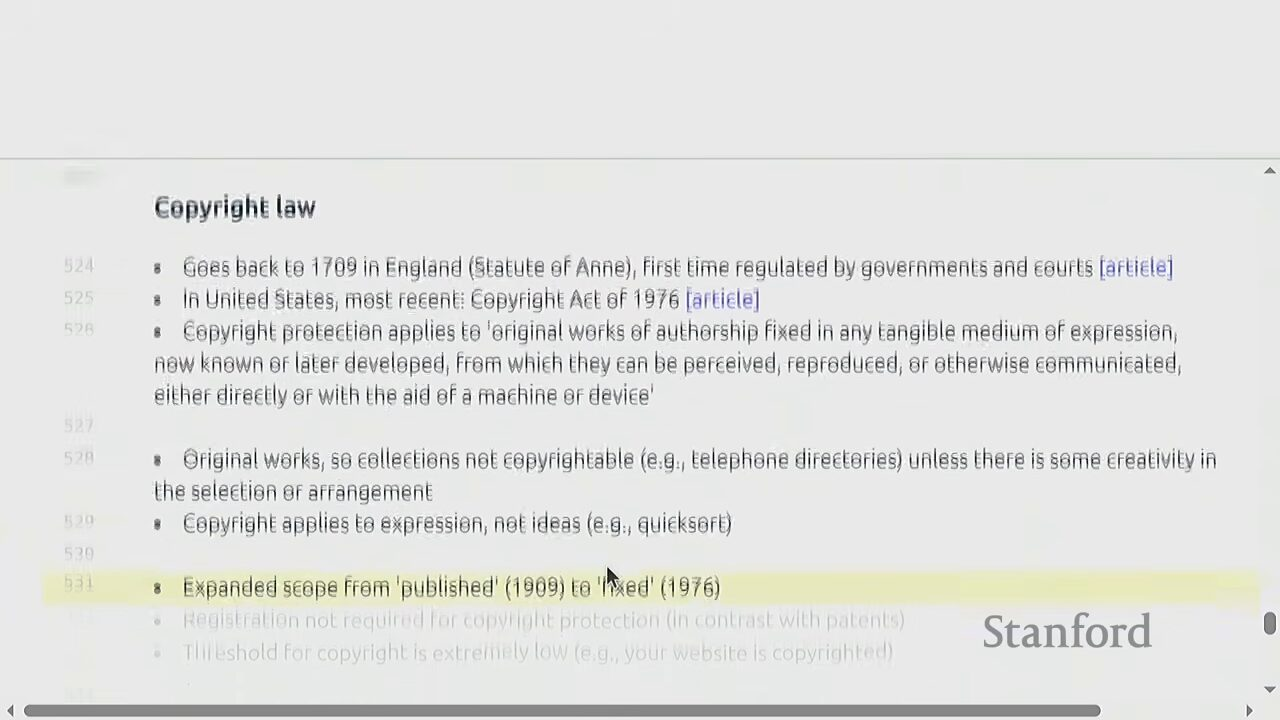
\includegraphics[width=0.92\textwidth]{figures/fig_23_copyright.jpg}
\caption{版权与合理使用的判定要素\protect\footnotemark}
\end{figure}
\footnotetext{视频画面时间区间：01:02:30--01:03:15。}

如今围绕生成式 AI 的诉讼大多关于版权。理解数据问题，必须先理解版权：

\begin{tcolorbox}[enhanced, colback=blue!5!white, colframe=blue!75!black, sharp corners, title=\textbf{版权（Copyright）基础}]
\begin{itemize}
\item \textbf{目的}：激励智力产品的创作。属于知识产权法的一部分（还有专利、商标、商业秘密）。
\item \textbf{美国 1976 版权法}：保护"固定在有形表达媒介上的\textbf{原创}作品"。关键是\emph{原创}——电话号码簿这种纯汇编不可版权（除非选择/编排有创意）。
\item \textbf{只保护表达，不保护思想}：算法不能版权，但\emph{代码}可以。
\item \textbf{无需注册即生效}：你把东西发到自己网站，它就自动受版权保护（即使没写"©"）。这和专利不同——专利不注册就没主张权。但起诉前需注册（注册费仅 \$65，远低于专利的数千美元）。
\item \textbf{期限}：75 年后过期进入公共领域。Gutenberg 的经典书大多已过期。
\end{itemize}
\end{tcolorbox}

\begin{importantbox}{核心现实}
\textbf{互联网上绝大多数内容都是版权的}。所以"是否版权"根本不是问题——\emph{问题是你能不能用}。两条路：\textbf{(1) 拿到许可（license）}；\textbf{(2) 诉诸合理使用（fair use）}。
\end{importantbox}

\subsection{许可（Licensing）}

许可路线有几种形式：

\begin{itemize}
\item \textbf{合同许可}：和创作者签合同（Google + Reddit 就是这种关系）。
\item \textbf{Creative Commons（CC）许可}：一种让版权作品能像公共领域一样自由分发的许可。作品\emph{仍然有版权}，只是作者预先授权了使用方式。Wikipedia 全部是 CC 许可，很多 YouTube 视频也是。CC 创立于约 20 年前，就是为了填补"公共领域"和"版权"之间的鸿沟，让创作者在不等 75 年的情况下允许他人使用。
\item 现在 Google+Reddit、OpenAI+Shutterstock、OpenAI+Stack Exchange 等都是付费许可关系。
\end{itemize}

\begin{warningbox}{许可路线的硬伤}
你\textbf{没法}为"整个互联网"拿到许可——你甚至不知道去找一个随机网站的谁谈。所以仅靠许可无法支撑大规模预训练。
\end{warningbox}

\subsection{合理使用（Fair Use）四要素}

\begin{figure}[H]
\centering
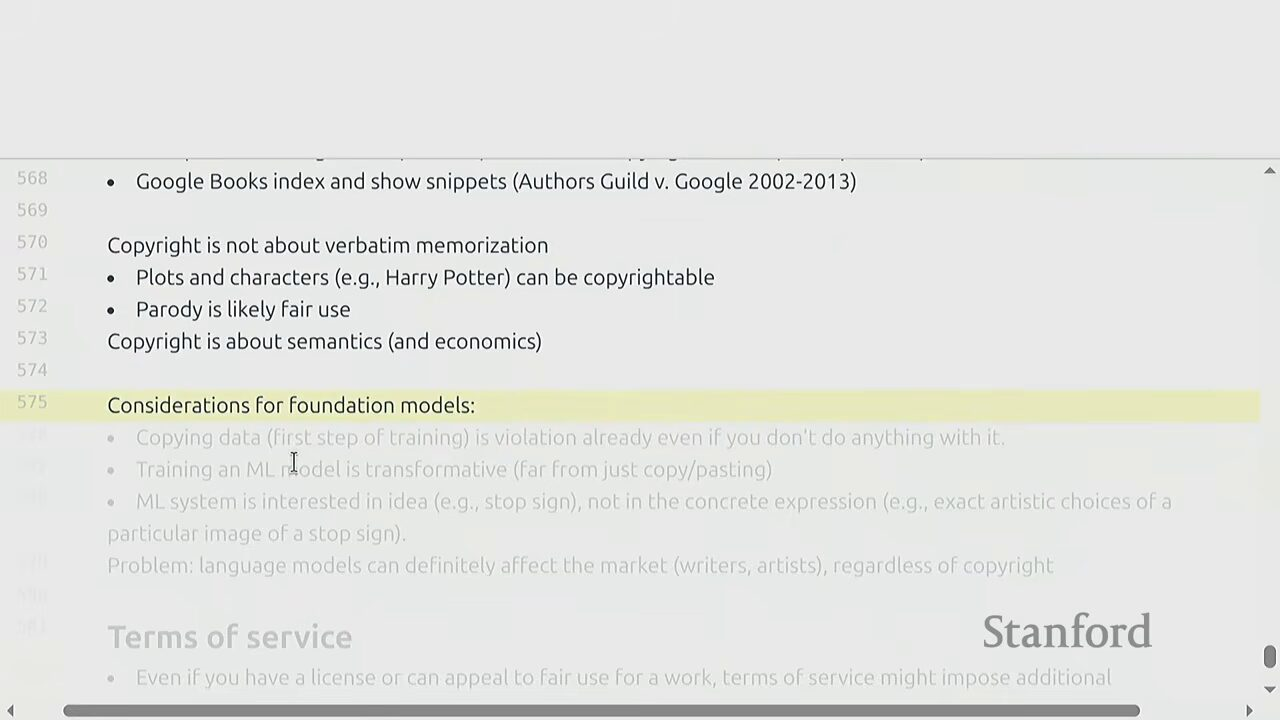
\includegraphics[width=0.92\textwidth]{figures/fig_24_fairuse.jpg}
\caption{训练作为"转化性使用"的法律争论\protect\footnotemark}
\end{figure}
\footnotetext{视频画面时间区间：01:08:00--01:08:45。}

合理使用允许你在没有许可的情况下使用版权内容，由\textbf{四要素}判定：

\begin{enumerate}
\item \textbf{使用的目的和性质}：教育性 vs. 商业性；是否\emph{转化}了原作品（而不是原样复制冒充自己的）。转化性使用更受青睐。
\item \textbf{原作品的性质}：事实性内容（如电话簿）更可能被判合理使用；虚构作品保护更强。
\item \textbf{使用的量和实质性}：只用一小段更安全——但对 LM 训练不适用，因为你通常想训全部。
\item \textbf{对市场的影响}：如果你的使用会\emph{替代}原作者的市场，不利；如果做完全不同的事，有利。（你看电影写摘要 = 合理使用；重新实现思想 = 没问题。）
\end{enumerate}

Google Books 长达十年的"展示片段是否合理使用"诉讼，最终判决\textbf{支持 Google}。

\begin{knowledgebox}{版权不仅是逐字复制}
即使几乎没有 n-gram 重叠，如果你拿走"哈利·波特"这个\emph{角色}并展开创作，\emph{也可能}侵犯版权。但如果你是\emph{戏仿}（parody），可能算合理使用。版权关乎语义、经济和内容，是个极其微妙的领域。
\end{knowledgebox}

\subsection{训练特有的法律问题}

把版权套到 ML 训练上，有几个独特的纠结：

\begin{tcolorbox}[enhanced, colback=red!5!white, colframe=red!75!black, sharp corners, title=\textbf{训练 vs. 版权：四个争论点}]
\begin{enumerate}
\item \textbf{复制这一步本身}：copyright 里就有"copy"。训练的第一步——\emph{复制数据}——技术上也已经是侵权，即使你什么都不做。
\item \textbf{训练是转化性的吗？}：许多人主张训练 LM 远不止复制粘贴，是高度转化的。但这让\emph{开源 + 开数据}变得棘手——你要展示训练数据就得托管它，而托管可能侵权。
\item \textbf{学的是思想还是表达？}：有人辩称 ML 关心的是"语言如何运作"这类通用知识（思想），而非特定作品（表达）。\emph{但模型会记忆}，且很容易从模型里提取训练数据。
\item \textbf{市场影响}：LM 无论版权与否，都可能影响内容创作者的市场。
\end{enumerate}
\end{tcolorbox}

\begin{warningbox}{许可 + 合理使用 都还不够}
即使你有许可、或能诉诸合理使用，你可能\emph{仍然无法合法获取数据}——因为\textbf{服务条款（ToS）}。比如 YouTube 有大量 CC 视频是公开的、CC 许可的，但你写脚本去批量下载 YouTube 视频，\emph{违反 YouTube 的服务条款}。这是平台层面的另一道门。
\end{warningbox}

\section{Mid-training 与 Post-training 数据}

这一节较短，且 mid/post 界限经常不清——都更关注"如何植入特定能力"而非笼统的"高质量"（尽管预训练也已经在考虑质量分类器了）。

\subsection{长上下文扩展}

顶级模型的上下文越来越长（Gemini、LLaMA 4 号称上千万 token）。由于 Transformer 对序列长度的复杂度是 \textbf{$O(N^2)$}（推理课讲过一些规避方法，但全注意力仍最好），人们\textbf{不会从头开始在长上下文上训练}，而是在 mid-training 阶段才引入，避免在模型还不行时浪费算力。

\begin{tcolorbox}[enhanced, colback=blue!5!white, colframe=blue!75!black, sharp corners, title=\textbf{长上下文的数据来源}]
需要创造\textbf{有长程依赖}的数据。\textbf{书籍}和\textbf{数学}是两个天然来源（上下文长、推理链长）。这类数据也可以\emph{合成}——用 LM 生成需要远距离引用的材料。
\end{tcolorbox}

注意力复杂度的代价可以用信息检索的视角理解。给定查询 $q$ 和一组键 $\{k_1, \dots, k_N\}$，标准注意力计算：

\[
\mathrm{ attn }(q) = \sum_{i=1}^{N} \frac{\exp(q \cdot k_i / \sqrt{d})}{\sum_{j=1}^{N} \exp(q \cdot k_j / \sqrt{d})}\, v_i
\]

每个查询要对所有 $N$ 个键算分数，于是总开销随 $N$ \textbf{平方}增长。这正是长上下文昂贵的根源，也是为什么把它推迟到 mid-training。

\subsection{任务格式化：FLAN 与 SuperNatural Instructions}

2022 年前后，社区把传统 NLP benchmark 转成统一格式以便微调。\textbf{SuperNatural Instructions} 让社区共建了 \textbf{1,600 个任务}并标准化成 prompt 格式。\textbf{FLAN}（2022 出、2023 论文）类似——"把所有 NLP 任务塞进指令跟随格式"。

\begin{practicebox}{任务格式化的优势与缺陷}
\textbf{优势}：一个模型能解决你所有喜欢的 NLP 任务，并从迁移学习中受益（这延续了 T5 的思路）。\\
\textbf{缺陷}：prompt 往往高度模板化——SuperNatural Instructions 里很多任务"看起来都一样"，并不"super"。这直接催生了后来更自然的指令跟随数据集。2022 年起，业界期望 LM 能处理任何一次性任务，"任务"这个概念本身开始消解。
\end{practicebox}

\subsection{合成数据的爆发（Post-training）}

开源社区在 post-training 上大量依赖\textbf{合成数据}，因为真人标注太贵：

\begin{itemize}
\item \textbf{Alpaca}：用 \textbf{self-instruct} 思想——prompt 一个 LM 生成示例，再用这些示例微调。
\item \textbf{Vicuna}：用用户在 ShareGPT（已废弃）上分享的对话。
\item 让 LM \emph{自我对话}： seeded 一些问题后让两个 LM 互相对话生成数据。
\item \textbf{Evol-Instruct}：拿一个问题，让 LM 把它变得更复杂。
\item 从 Common Crawl 识别 quiz 站点，用 LM 抽取 QA 对。
\item \textbf{OpenHermes}：各种数据集的大杂烩（前面 DCLM 用它做正例）。
\item \textbf{LLaMA 2 Chat}：数据集不公开，但用了\emph{人工标注员}写高质量指令数据，论文声称这优于数百万开源样本——不过他们本可以通过更少标注 + 更多 RLHF 省钱。
\item \textbf{Llama-Nemotron post-training data}：含 WildChat 等公开数据 + 从各模型合成 + 推理轨迹（受 R1 启发）。
\end{itemize}

\begin{tcolorbox}[enhanced, colback=yellow!10!white, colframe=yellow!80!black, sharp corners, title=\textbf{合成数据的三个来源谱系}]
\begin{enumerate}
\item \textbf{蒸馏自 GPT-4}：最简单。但 OpenAI 的 ToS \emph{禁止}用 GPT-4 造数据训练竞争模型——学术研究可以，商用不行。
\item \textbf{蒸馏自 open-weight 模型}：许可更宽松，可以自由蒸馏（Llama 可能有些限制，但比 OpenAI 宽松）。
\item \textbf{纯人工标注}：最贵最慢，而且要当心标注员偷偷用 GPT-4 生成数据糊弄你。
\end{enumerate}
\end{tcolorbox}

\section{总结}

\begin{figure}[H]
\centering
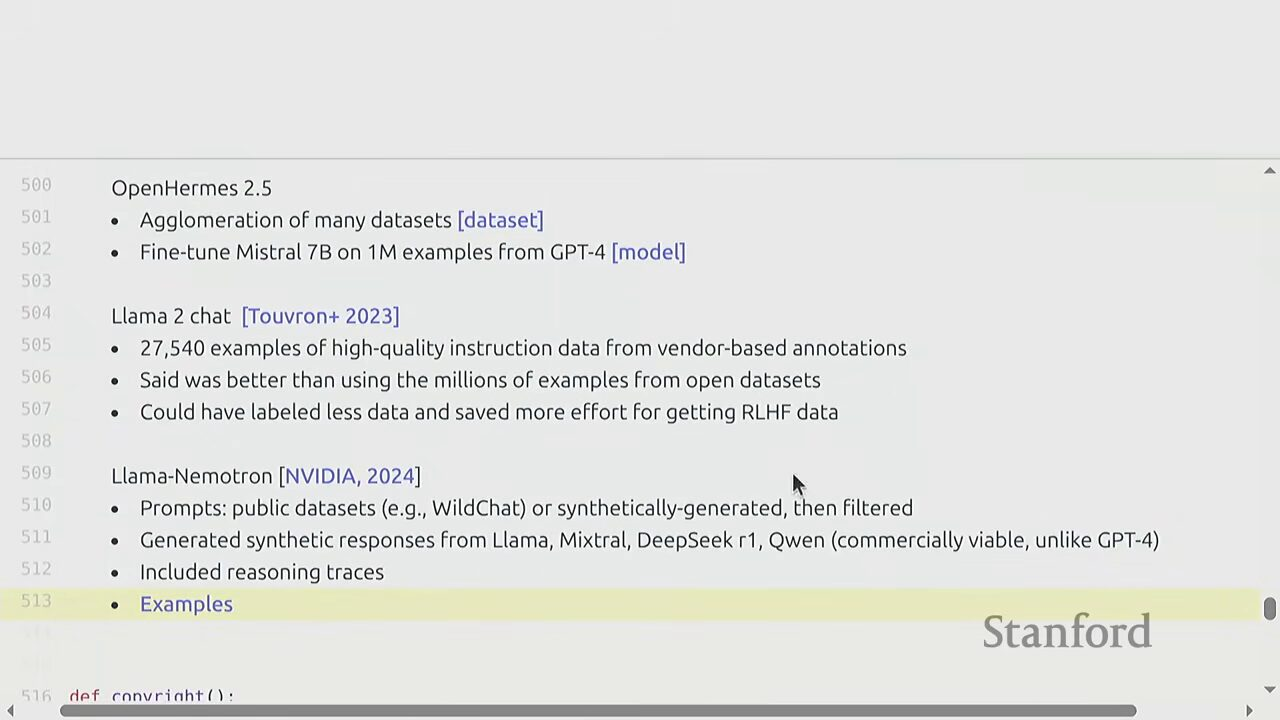
\includegraphics[width=0.92\textwidth]{figures/fig_25_summary.jpg}
\caption{总结：数据不会从天而降\protect\footnotemark}
\end{figure}
\footnotetext{视频画面时间区间：01:17:00--01:17:45。}

\begin{importantbox}{五个核心论点}
\begin{enumerate}
\item \textbf{数据不会从天而降}。GitHub、Wikipedia 这些是\emph{活的在线服务}——要训练得先拿到 raw dump，但 raw dump 太大、太噪、甚至不是 tokens，必须经过大量处理（质量过滤、去重等）才能用。
\item \textbf{数据是模型差异的真正来源}。架构基本都是 Transformer 风格、通用到行为差别不大；真正驱动质量的是数据（前提是你能训得动、拟合得了数据）。
\item \textbf{存在大量法律与伦理问题}。版权只是冰山一角，还有更多没讲的。
\item \textbf{这个领域是一片混乱}。高度启发式，\emph{意味着有大量改进机会}。
\item \textbf{范式在转向}：从"避免用模型过滤"到"在回路里用模型"，质量分类器 + LM 改写/扩写已成为主流。
\end{enumerate}
\end{importantbox}

\subsection{贯穿全讲的几条主线}

回看从 BERT 到 Nemotron-CC 的演化，有几条反复出现的主线值得记牢：

\begin{knowledgebox}{数据工程的几条元原则}
\begin{itemize}
\item \textbf{代理选择决定上限}：CCNet 用 Wikipedia、GPT-3 用 WebText+Wiki、DCLM 用 OpenHermes+ELI5、Nemotron 用教育价值。你定义的"好"塑造了你能捞到的数据。
\item \textbf{链接结构是金矿}：WebText 的 Reddit karma、LLaMA 的"被 Wiki 引用"——间接质量信号往往比直接判断更鲁棒。
\item \textbf{规则 vs. 模型是辩证的}：C4/RefinedWeb 的纯规则路线与 CCNet/GPT-3 的模型路线各有优劣；今天的主流是\emph{两者结合}（规则粗筛 + 模型精排）。
\item \textbf{去重不可省}：几乎每个数据集都做了去重（exact + MinHash fuzzy），因为互联网天然充满重复。
\item \textbf{量与质的张力}：DCLM 要质（240T$\to$3.8T），Nemotron 要量（6.3T + LM 改写）——取决于你的模型规模和训练预算。
\end{itemize}
\end{knowledgebox}

\subsection{配套阅读与延伸}

\begin{tabular}{p{7cm}p{6cm}}
\toprule
\textbf{论文 / 资源} & \textbf{对应知识点} \\
\midrule
BERT (Devlin+ 2018) & Books + Wikipedia 时代 \\
WebText / GPT-2 (Radford+ 2019) & Reddit karma 筛选 \\
C4 / T5 (Raffel+ 2019) & 纯启发式规则清洗 \\
CCNet (Wenzek+ 2019) & Wikipedia 5-gram 质量过滤 \\
GPT-3 (Brown+ 2020) & 质量分类器兴起 \\
The Pile (Gao+ 2020) & 22 领域策展 \\
MassiveText (Rae+ 2021) & Gopher rules + SafeSearch \\
LLaMA (Touvron+ 2023) & "被 Wikipedia 引用"分类器 \\
RefinedWeb (Penedo+ 2023) & 纯规则 + 模糊去重 \\
FineWeb (Hugging Face 2024) & 15T 轻度过滤 \\
DOLMA (Soldaini+ 2024) & OLMo 多源组合 \\
DataComp / DCLM (Li+ 2024) & 240T$\to$3.8T 竞赛 \\
Nemotron-CC (Nvidia 2024) & 教育评分 + LM 改写 \\
\bottomrule
\end{tabular}

%% --- 正文内容结束 ---

\end{document}
